\documentclass[twocolumn,11pt,a4paper]{article}

% Essential packages
\usepackage{lipsum}          % For dummy text
\usepackage{graphicx}        % For including images
\usepackage{amsmath}         % For mathematical equations
\usepackage{amsthm}          % For theorems
\usepackage{booktabs}        % For better tables
\usepackage{microtype}       % For better typography
\usepackage[english]{babel}  % For language settings
\usepackage{geometry}        % For page layout
\usepackage{titlesec}        % For section title formatting
\usepackage{enumitem}        % For customized lists
\usepackage{placeins}        % Add this package

% Chinese font support - add these packages
\usepackage{fontspec}
\usepackage{xeCJK}

% Chinese font configuration
\setmainfont{Sarasa Gothic TC} % Or specify another suitable font like Noto Serif CJK TC
\setCJKmainfont{Sarasa Gothic TC} % Or specify another suitable font like Noto Sans CJK TC
\setCJKsansfont{Sarasa Gothic TC} % Or specify another suitable font like Noto Sans CJK TC
\setCJKmonofont{Sarasa Gothic TC} % Or specify another suitable font like Noto Sans Mono CJK TC

% Page layout
\geometry{
  margin=1.5cm,
  top=1.5cm,
  bottom=2cm,
}

% Set paragraph indentation
\setlength{\parindent}{2em} % Sets indentation to approximately 2 characters width

% Title formatting
\titleformat{\section}
  {\normalfont\large\bfseries}{\thesection}{1em}{}
\titleformat{\subsection}
  {\normalfont\normalsize\bfseries}{\thesubsection}{1em}{}
\titleformat{\subsubsection}
  {\normalfont\normalsize\itshape}{\thesubsubsection}{1em}{} % Added for subsubsection

% Colors for hyperlinks - place after fontspec packages
\usepackage{hyperref}
\hypersetup{
  colorlinks=true,
  linkcolor=blue,
  filecolor=magenta,
  urlcolor=cyan,
  citecolor=green,
}

% Begin document
\begin{document}
% Title page (takes full width)
\twocolumn[
    \begin{@twocolumnfalse}
        \centering
        \vspace{1.5cm}
        {\LARGE\bfseries 軟體工程期中考試書面報告\par}
        \vspace{0.3cm}
        {\small\textit{軟體工程中大語言模型軟體 Kuwa + TAIDE + RAG 和 QCI\&AI 軟硬體整合的應用}\par}
        \vspace{1cm}

        % 作者資訊區塊
        {\large{黃毓峰 - S11159005}\par}
        \vspace{0.3cm}
        {\large 國立臺南大學 資訊工程學系\par}
        \vspace{0.3cm}
        {\large a288235403@gmail.com\par}
        \vspace{0.3cm}
        {\large 指導教授:李健興 教授\par}
        \vspace{0.5cm}

        {\large \today\par}
        \vspace{1cm}
    \end{@twocolumnfalse}
]

% Abstract
\section*{摘要}
本報告目的是整合軟體工程 (Software Engineering) 
的核心概念與量子計算智慧暨人工智慧 (Quantum Computational Intelligence \& 
Artificial Intelligence, QCI\&AI) 學習工具的實作經驗,
以建立一個兼具理論與實務的綜合學習框架。
透過回顧李允中教授的 Software Engineering 教科書前四章的關鍵知識點,
並詳述 Kuwa 平台、大型語言模型 (Large Language Model, LLM) API 與本地模型部署的過程
,以及檢索增強生成 (Retrieval-Augmented Generation, RAG) 功能的應用,
本報告展示了如何將 Software Engineering 原則應用於 QCI\&AI 領域的學習與探索,特別是在資料收集、
推論模型建立與微調模型的學習階段中。本報告也強調了 Software Engineering 在 QCI\&AI 學習中的重要性,
並將 Software Engineering 的原則應用於資料收集、推論模型建立和微調模型的學習階段。
\linebreak \linebreak 
\noindent \textbf{關鍵字:} 軟體工程、量子計算智慧、人工智慧、大型語言模型、檢索增強生成、TAIDE

\section*{Abstract}
The purpose of this report is to integrate the core concepts of Software 
Engineering with practical experience in implementing Quantum 
Computational Intelligence \& Artificial Intelligence (QCI\&AI) learning tools, 
establishing a comprehensive learning framework that combines theory and practice. 
By reviewing the key knowledge points from the first four chapters 
of Professor Li Yun-Chung's software engineering textbook
, detailing the deployment process of the Kuwa platform,
Large Language Model (LLM) APIs, and local models, 
and the application of Retrieval-Augmented Generation 
(RAG) functionality, this report demonstrates how  
software engineering principles can be applied to  
learning and exploration in the QCI\&AI field,  
particularly during the learning stages of data collection,  
inference model building, and model fine-tuning.  
The report also emphasizes the importance of software engineering in QCI\&AI learning and applies software engineering principles to the learning stages of data collection, inference model building, and model fine-tuning.
\linebreak \linebreak
\noindent \textbf{Keywords:} Software Engineering, Quantum Computational Intelligence, Artificial Intelligence, Large Language Models, Retrieval-Augmented Generation, TAIDE

\section{Introduction}
隨著資訊科技的飛速發展,軟體系統已滲透到現代社會的各個角落,Software Engineering 的重要性不言喻。同時,Artificial Intelligence (AI) 與量子計算 (Quantum Computing) 的融合,催生了量子計算智慧 (Quantum Computational Intelligence, QCI) 這一新興領域。本報告的目的為結合 Software Engineering 的核心理論與 QCI\&AI 技術及 LLM 應用的實務經驗,建立一個綜合性的學習與實踐框架。

首先,我們將簡要回顧李允中教授《軟體工程》教科書前四章的核心內容 \cite{li2013ch1, li2013ch2, li2013ch3, li2013ch4}。第一章「軟體危機與流程」探討了 Software Crisis 的成因、Software Engineering 的本質性挑戰,並介紹了基本的軟體開發活動 (Software Development Activities) 與主流的 Software Process Models,如瀑布模型 (Waterfall Model)、V模型 (V-Model)、統合流程 (Unified Process)、極限製程 (Extreme Programming, XP) 及 Scrum 等 \cite{li2013ch1}。
% Placeholder for textbook figure from CH1
\begin{figure}[htbp]
    \centering
    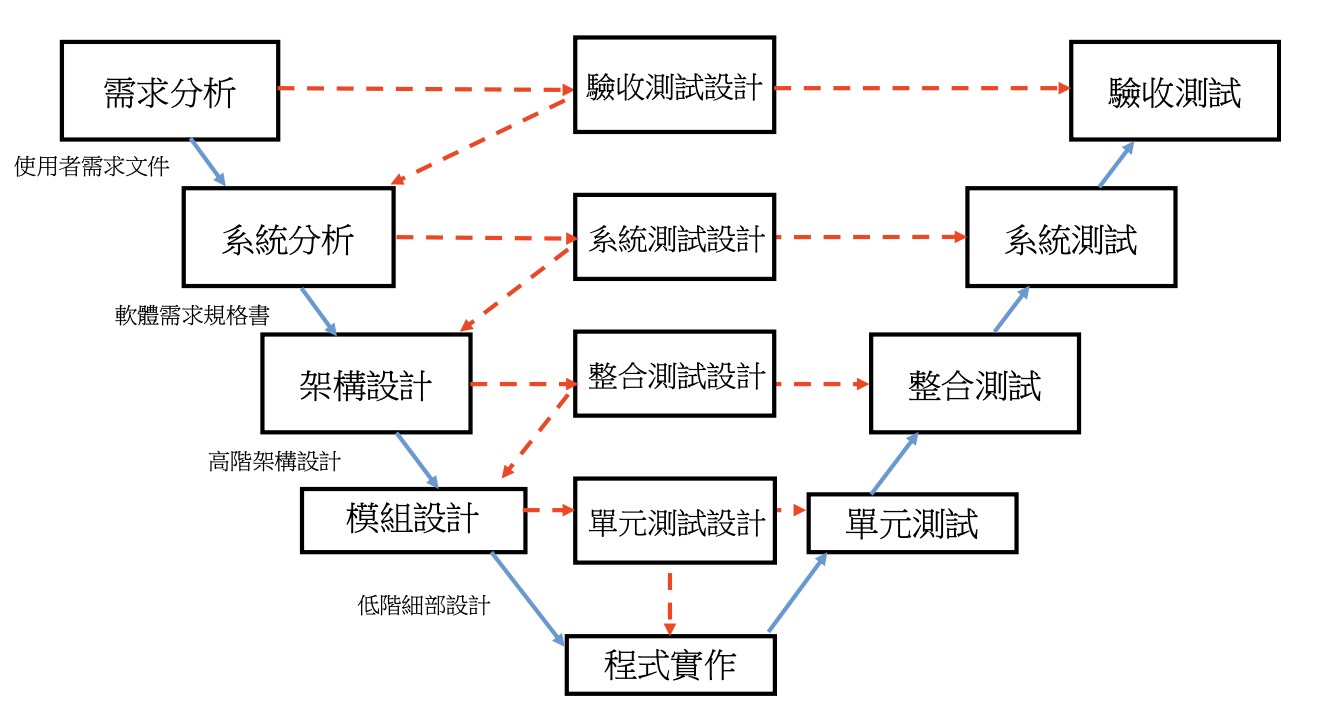
\includegraphics[width=0.45\textwidth]{res/image/v_model.png}
    \caption{Software Process Model 示例 (來源:\cite{li2013ch1})}
    \label{fig:textbook_ch1_fig}
\end{figure}
\FloatBarrier

第二章「需求工程」闡述了 Requirements Engineering 的完整過程,包括需求的種類(如 User Requirements, System Requirements, Functional Requirements, Non-functional Requirements)、需求擷取 (Requirements Elicitation)、需求分析 (Requirements Analysis)(涵蓋 Data Flow Analysis, Entity Relationship Analysis 等)、需求規格化 (Requirements Specification)、需求確認 (Requirements Validation) 及需求管理 (Requirements Management) \cite{li2013ch2}。
% Placeholder for textbook figure from CH2
\begin{figure}[htbp]
    \centering
    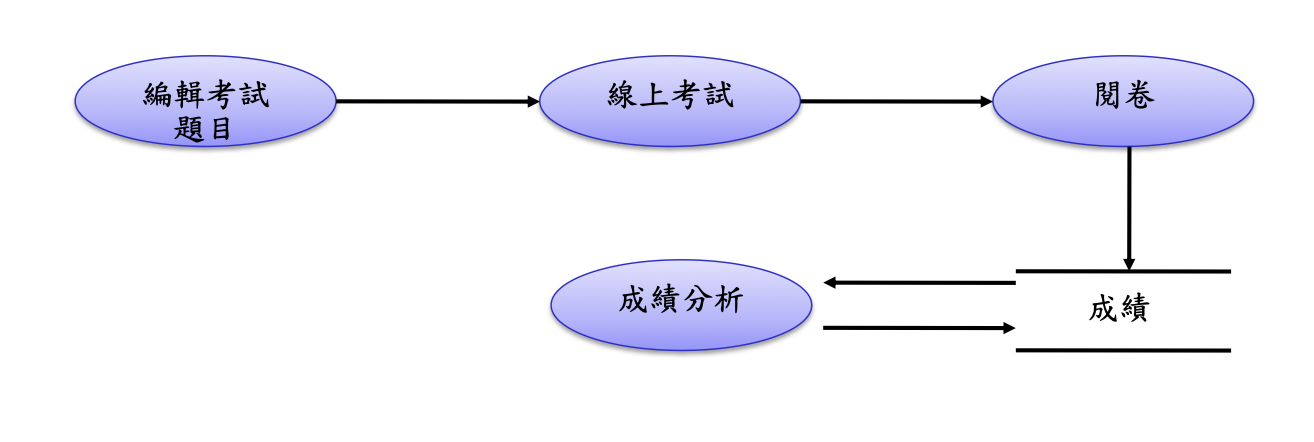
\includegraphics[width=0.45\textwidth]{res/image/DFD.png} % Example
    \caption{Requirements Engineering 圖示示例 (來源:\cite{li2013ch2})}
    \label{fig:textbook_ch2_fig}
\end{figure}
\FloatBarrier

第三章「物件導向軟體開發」深入介紹了物件導向 (Object-Oriented, OO) 的基本概念、UML 塑模語言、OO Software Development 流程(分析、設計、建構),
並探討了使用者需求塑模 (User Requirement Modeling)、
OO Analysis 及 OO Design 方法 \cite{li2013ch3}。


第四章「軟體設計」則討論了軟體設計 (Software Design) 
的核心原則(如抽象化 (Abstraction), 模組化 (Modularity), 
內聚力 (Cohesion), 耦合力 (Coupling))、架構設計 (Architectural Design) 
樣式、Software Design 策略(功能導向 (Function-Oriented) 
與 OO Design)、以及服務導向架構 (Service-Oriented Architecture, SOA) 
等進階主題 \cite{li2013ch4}。這些 Software Engineering 理論為後續的實作應用提供了堅實的基礎。

\begin{figure}[htbp]
    \centering
    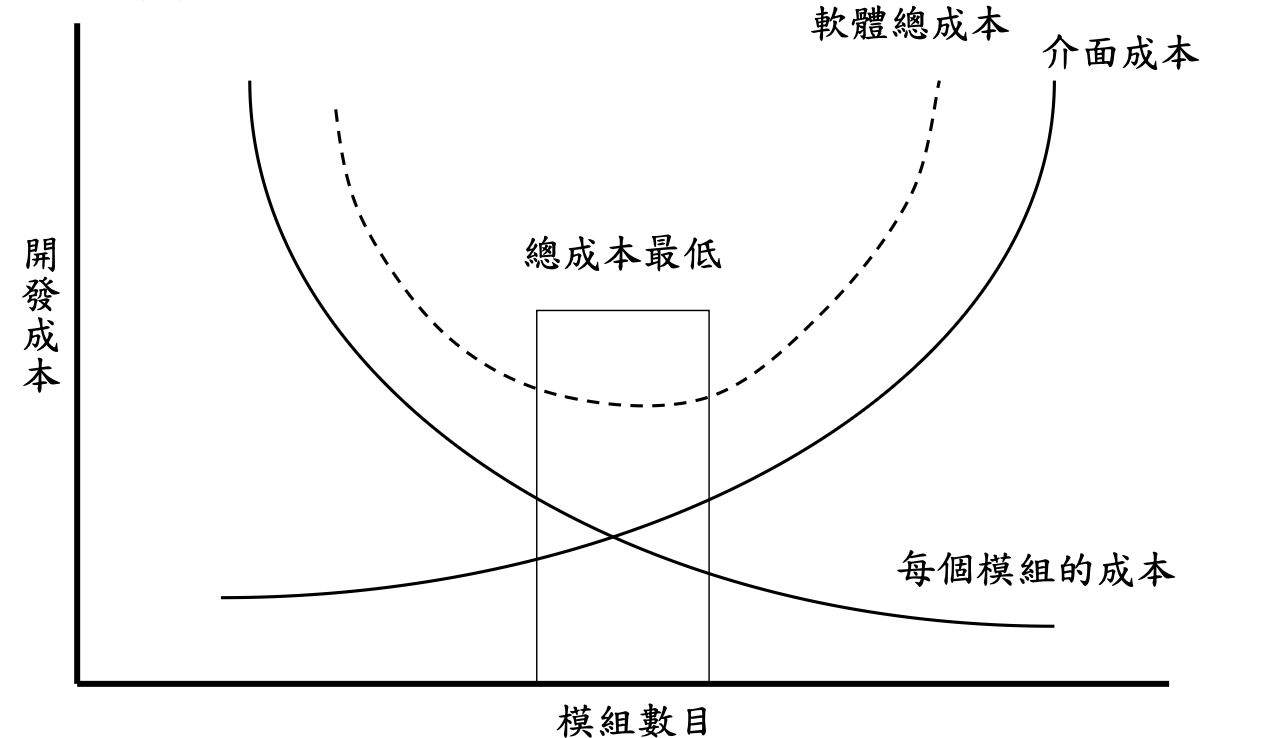
\includegraphics[width=0.45\textwidth]{res/image/model_and_price.png}
    \caption{模組與成本關係圖 (來源:\cite{li2013ch4})}
    \label{fig:model_and_price}
\end{figure}
\FloatBarrier

本報告接下來將詳述 QCI\&AI 軟硬體整合學習工具以及 Kuwa 平台結合 TAIDE\cite{llama_taide} 模型與 RAG 功能的實作細節。
第二節「軟體需求工程, LLM」將聚焦於 KUWA+TAIDE+RAG 的操作步驟與實作結果,展示如何應用 Requirements Engineering 概念於 LLM 環境的建置與使用。
第三節「軟體專案規劃, QCI\&AI軟硬體生活應用」將闡述 QCI\&AI 軟硬體工具的操作流程與實作成效,並探討其在生活中的潛在應用,體現 Software Project Planning 的初步構想。
第四節「軟體工程LLM軟體應用 (Macro/Meso/Micro)」與第五節「軟體工程QCI\&AI軟硬體整合應用 (Macro/Meso/Micro)」將分別從不同層次探討 LLM 與 QCI\&AI 技術在 Software Engineering 實踐中的應用潛力,並展示相關的時程規劃。
最後,第六節「生成式AI對我學習軟體工程分析」將分享個人在使用生成式 AI 工具學習 Software Engineering過程中的心得體會與反思。
透過理論回顧與實務操作的結合,本報告期望為 Software Engineering 學習者提供一個整合性的視角,以應對 AI 與 QCI 技術融合帶來的機遇與挑戰。

\section{軟體需求工程, LLM (KUWA+TAIDE+RAG 操作步驟及實作結果)}
本節詳細介紹 Kuwa 平台結合 TAIDE 模型及 RAG 功能的安裝設定流程與初步實作結果。此過程可視為一個小型軟體專案的 Requirements Engineering 與初期建置階段,目標是建立一個可用的 LLM 互動與知識增強環境。

\subsection{Kuwa 平台安裝與設定}
Kuwa GenAI OS (以下簡稱 Kuwa) 是一個提供與 LLM 互動環境的平台。其安裝方式因操作系統而異。

\textbf{Windows 環境:} % (內容參考先前版本,已符合術語格式)
根據提供的 Windows 版本安裝指引 (v.0.9) 和 KUWA TAIDE v0.2.0 安裝手冊,主要步驟包括:
\begin{enumerate}[noitemsep, topsep=0pt]
    \item \textbf{環境準備}:安裝 Microsoft Visual C++ 可轉散發套件,以及(若使用 GPU)對應版本的 NVIDIA CUDA Toolkit。
    \item \textbf{下載 Kuwa}:從指定網址下載對應 CPU 或 GPU (CUDA 版本) 的 `.exe` 執行檔,或從 GitHub 獲取源碼。
    \item \textbf{執行與啟動}:執行 `.exe` 文件或相關啟動腳本 (`build.bat`, `start.bat`)。系統會啟動本地伺服器,通常可通過瀏覽器訪問 `http://localhost:8080`。
\end{enumerate}

\textbf{Linux 環境 (基於 Docker):} % (內容參考先前版本,已符合術語格式)
另一種常見方式是在 Linux 環境(如 Ubuntu VM)中使用 Docker 進行部署。此方法更靈活但也更複雜,尤其在需要利用主機 GPU 資源時:
\begin{enumerate}[noitemsep, topsep=0pt]
    \item \textbf{環境準備}:建立虛擬機 (如使用 QEMU/KVM),配置 GPU Passthrough(涉及 IOMMU 啟用、`vfio-pci` 模組加載、啟動/停止掛鉤腳本設定等複雜步驟),並在 VM 內安裝 Docker、NVIDIA 驅動及 NVIDIA Container Toolkit。
    \item \textbf{下載與配置 Kuwa}:克隆 `genai-os` GitHub 倉庫。
    \item \textbf{構建與運行容器}:根據需求拉取或構建 Docker 鏡像(例如,為 GPU 使用拉取 `kuwaai/model-executor:v0.3.4-cu121` 並標記為 `latest`),並使用 Docker Compose(通過修改 `run.sh` 執行多個 `.yaml` 配置文件)來啟動 Kuwa 的各個服務容器。
\end{enumerate}
不論何種安裝方式,Kuwa 平台都提供了一個儀表板 (Dashboard),包含聊天 (Chat) 和房間 (Room) 等功能。

\subsection{雲端 LLM API 整合 (Gemini Pro)}
% (內容參考先前版本,已符合術語格式)
Kuwa 平台支援串接外部的 LLM API,例如 Google Gemini Pro。整合步驟如下:
\begin{enumerate}[noitemsep, topsep=0pt]
    \item \textbf{獲取 API 金鑰}:前往 Google AI Studio (\url{ai.google.dev}) 申請並獲取 Gemini API 金鑰。
    \item \textbf{配置 Kuwa}:在 Kuwa 平台的界面中,通常在個人設定 (Profile) 或相關設定頁面,找到 API 金鑰輸入欄位,將獲取的 Gemini API 金鑰填入。
    \item \textbf{測試連接}:保存設定後,在 Chat 界面選擇 Gemini Pro 模型,發送訊息進行測試,確認是否能成功接收回覆。
\end{enumerate}

\subsection{本地 GGUF 模型部署 (TAIDE LLaMA.cpp)}
% (內容參考先前版本,已符合術語格式,加入TAIDE)
Kuwa 也支援透過 Llama.cpp 等後端運行本地的 LLM,例如 TAIDE 的 GGUF (GPT-Generated Unified Format) 版本。部署方式根據 Kuwa 的安裝環境有所不同:

\textbf{Windows 環境 (基於 \texttt{env.bat}):}
\begin{enumerate}[noitemsep, topsep=0pt]
    \item \textbf{下載 TAIDE GGUF 模型}:從相關模型庫下載 TAIDE 的 GGUF 格式模型檔案。
    \item \textbf{配置環境變數}:編輯 Kuwa 目錄下的 \texttt{env.bat} 文件。找到 \texttt{gguf\_path} 相關的行,取消註解並填寫下載的 TAIDE GGUF 模型檔案的完整路徑。
    \item \textbf{重新啟動 Kuwa}:關閉並重新執行 `start.bat`。
    \item \textbf{選擇模型}:在 Kuwa Dashboard 的模型選擇列表中,應會出現 LLaMA.cpp Model (TAIDE) 或類似選項。
\end{enumerate}

\textbf{Linux 環境 (基於 Docker Compose):}
\begin{enumerate}[noitemsep, topsep=0pt]
    \item \textbf{下載 TAIDE GGUF 模型}:同上。
    \item \textbf{創建 Docker Compose 配置}:在 \texttt{compose} 目錄下為 TAIDE 模型創建一個新的 \texttt{.yaml} 文件。在此文件中定義服務,指定使用 \texttt{kuwaai/model-executor} 鏡像,設置環境變數(如 \texttt{EXECUTOR\_TYPE: llamacpp}, 模型名稱如 \texttt{TAIDE-LLAMA3-8B-CHAT-GGUF} 等),並通過 volumes 將本地模型文件映射到容器內的 \texttt{/var/model/} 路徑。
    \item \textbf{修改啟動腳本}:編輯 `run.sh` 文件,在 `confs` 數組中加入新創建的 Compose 文件名。
    \item \textbf{重新啟動 Kuwa}:執行 `./run.sh`。
    \item \textbf{選擇模型}:在 Kuwa Dashboard 中選擇新配置的 TAIDE 模型。
\end{enumerate}

\subsection{RAG 功能應用}
% (內容參考先前版本,已符合術語格式)
Retrieval-Augmented Generation (RAG) 是 Kuwa 的一項重要功能。在 Windows 環境下設定 RAG 的基本步驟如下:
\begin{enumerate}[noitemsep, topsep=0pt]
    \item \textbf{環境準備}:可能需要運行 Kuwa 目錄下的 \texttt{tool.bat} 切換模式及安裝特定 Python 依賴 (`numpy==1.24.4`, `faiss-cpu==1.7.4`)。
    \item \textbf{構建知識庫}:準備包含知識文件的資料夾,拖曳到 Kuwa 的「Construct RAG」捷徑以建立向量索引。
    \item \textbf{配置 RAG Bot}:進入 Kuwa Dashboard 的「Store」,選擇建立的 RAG Bot,在「Model config file」中指定用於生成的 LLM (例如本地 TAIDE 模型)。
    \item \textbf{開始問答}:與配置好的 RAG Bot 互動。
\end{enumerate}

\subsection{實作結果與安裝影片}
KUWA+TAIDE+RAG 系統成功在 Windows 環境下搭建完成。本地 TAIDE GGUF 模型能夠順利加載並透過 Kuwa 界面進行互動。RAG 功能允許上傳自定義文檔,LLM能夠基於這些文檔內容回答問題,顯著提升了回答的相關性和準確性。詳細的安裝與操作過程已錄製成影片。


% Placeholder for KUWA+TAIDE+RAG result figure
\begin{figure}[htbp]
    \centering
    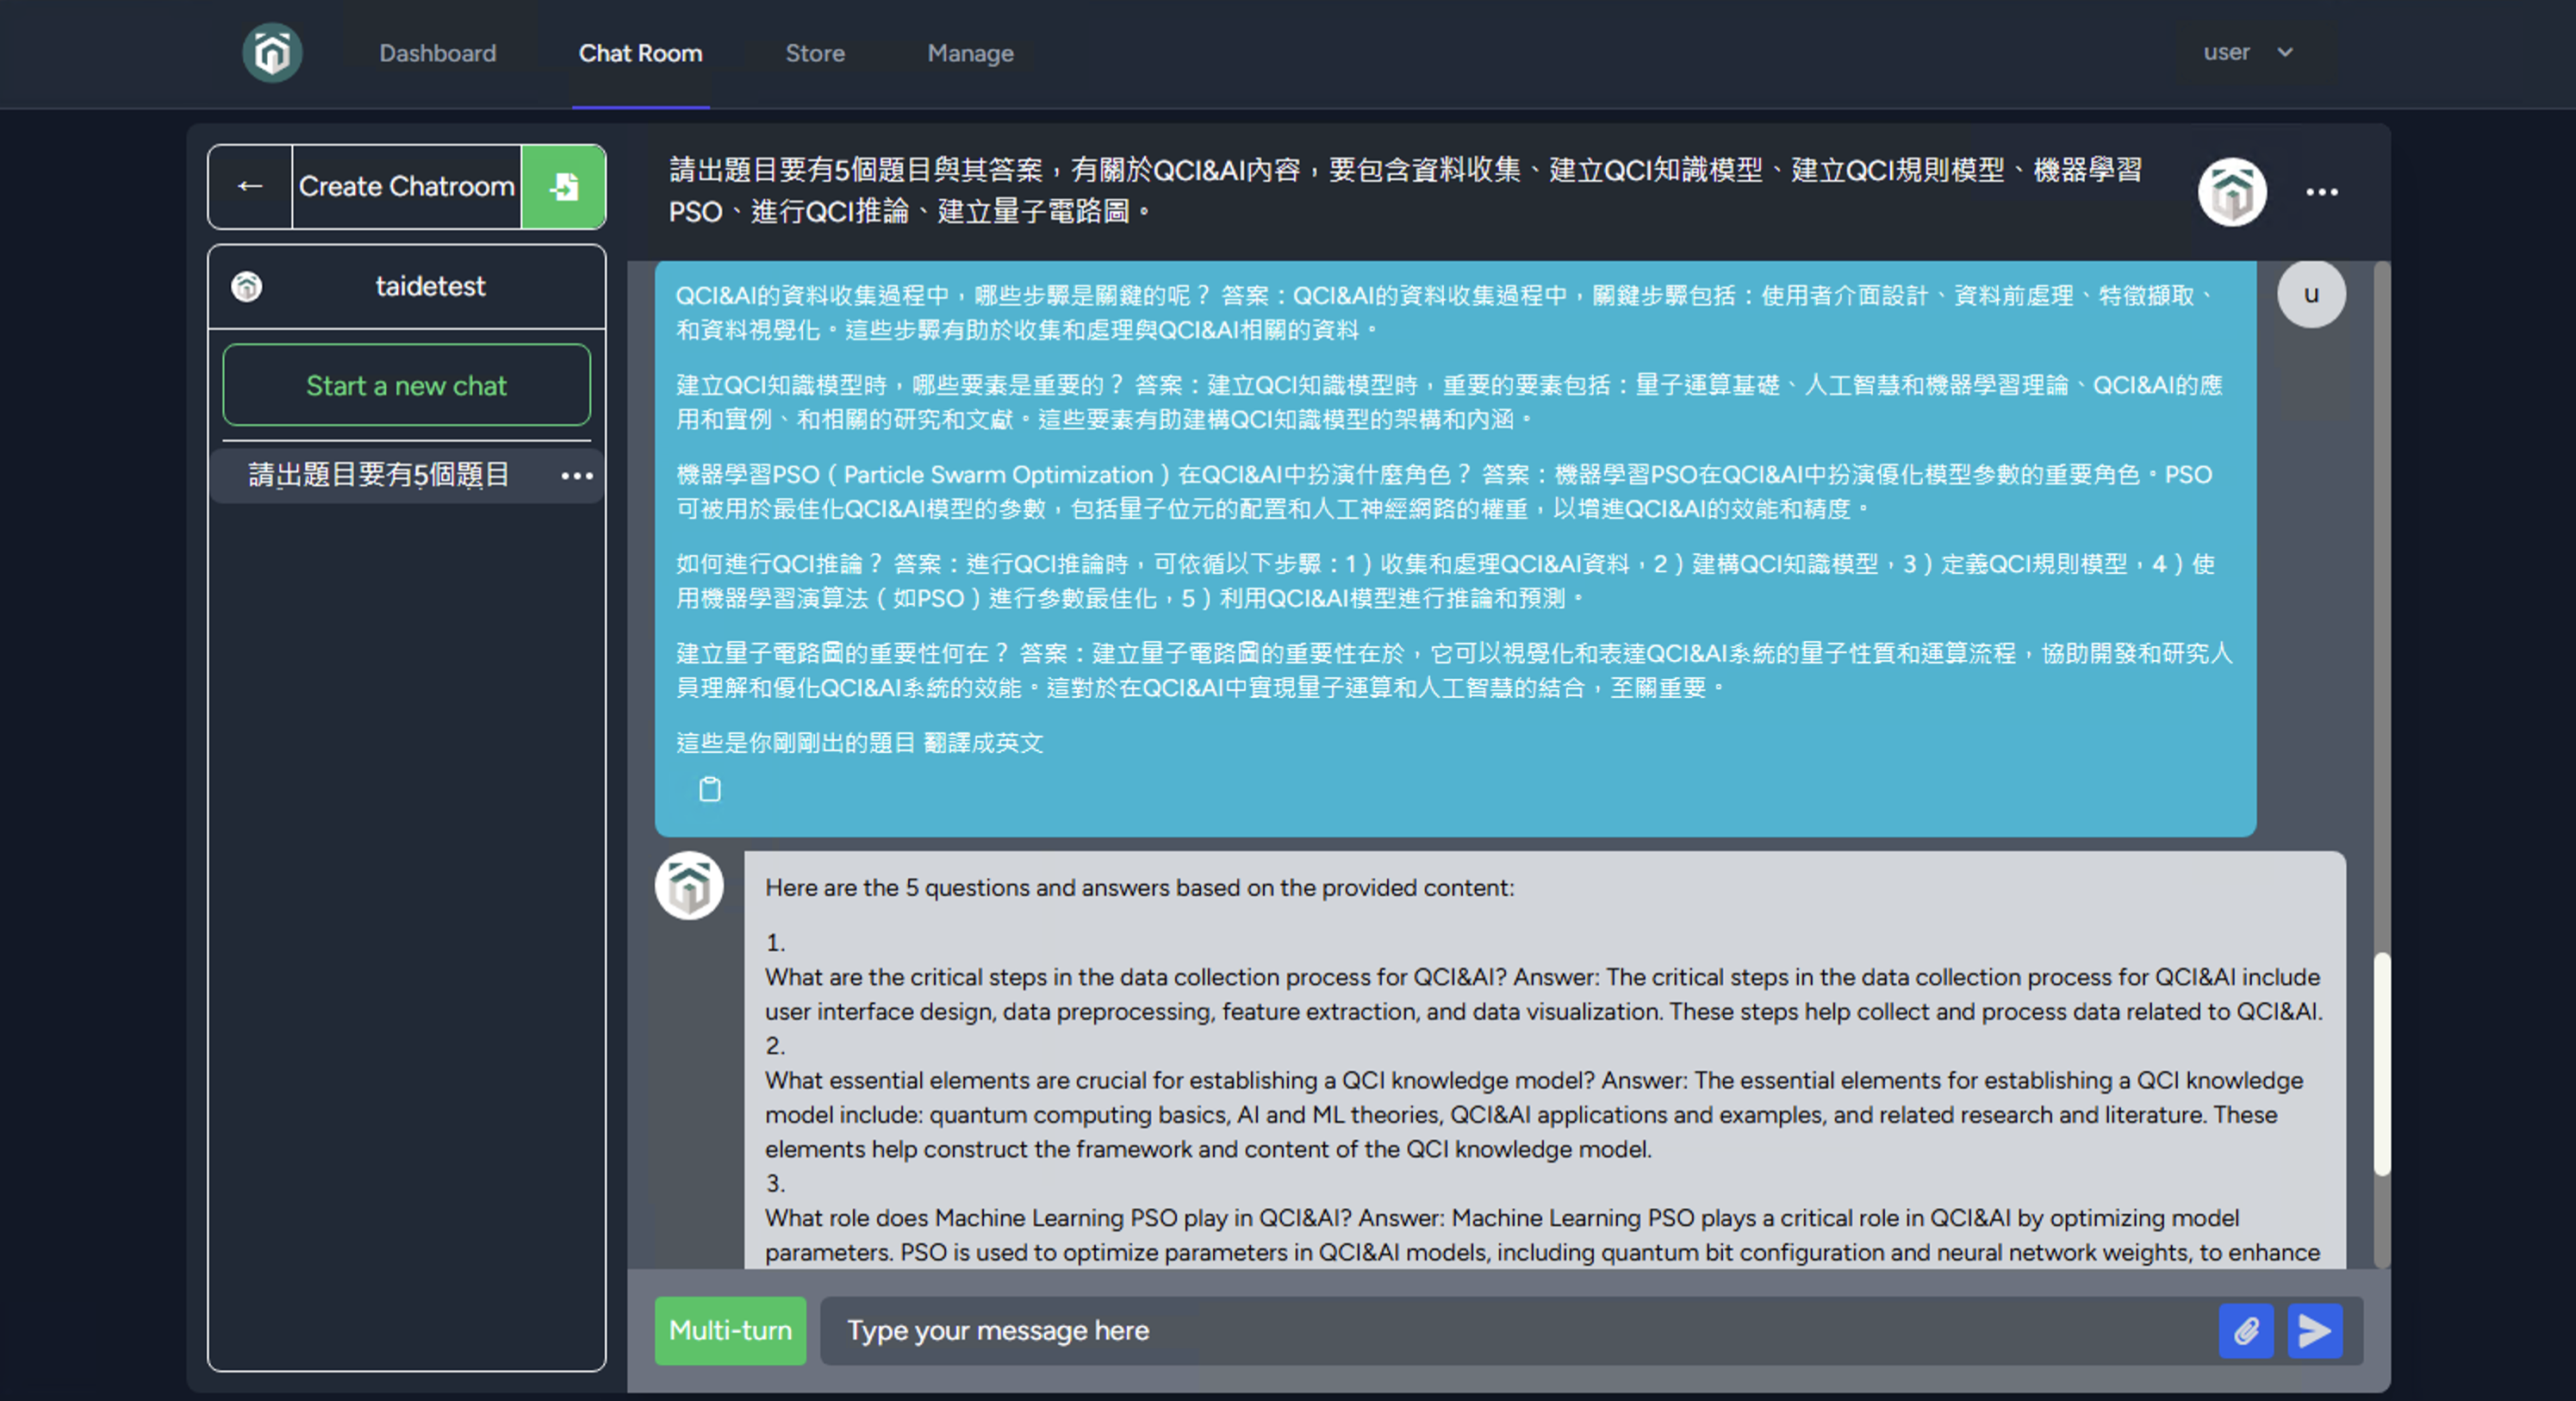
\includegraphics[width=0.45\textwidth]{res/image/taide_chat.png} % Example
    % \fbox{\parbox[c][15em][c]{0.45\textwidth}{\centering 預留位置: \\ KUWA+TAIDE+RAG \\ 實作結果截圖 \\ (例如:RAG問答界面)}}
    \caption{KUWA+TAIDE+RAG 實作結果示例}
    \label{fig:kuwa_rag_result}
\end{figure}
\FloatBarrier

\section{軟體專案規劃, QCI\&AI軟硬體生活應用}
本節闡述 QCI\&AI 軟硬體學習工具的操作步驟與實作成效,並初步探討其在生活應用方面的 Software Project Planning 概念。此工具的開發與應用本身可視為一個小型 Software Project。

\subsection{QCI\&AI 軟硬體環境設定與資料蒐集}
% (內容參考先前版本,已符合術語格式)
\begin{itemize}
    \item 下載並安裝 Thonny 4.1.7 軟體環境。
    \item 設定 Thonny 使用 MicroPython (generic) 模式,並選取正確的通訊埠 (COM Port)。
    \item 將 QCI\&AI 學習工具透過 USB 接上個人電腦,並啟動工具。
    \item 使用 Thonny 執行 \texttt{QCIGAIModel\_DataCollection.py} 進行 Data Collection,擷取影像及距離 (Distance)、光線 (Light) 資訊。
\end{itemize}

\subsection{模糊集合與模糊系統實作}
% (內容參考先前版本,已符合術語格式)
利用 QCI\&AI 學習工具與 KWS AI 平台進行 Data Collection 與處理:
\begin{itemize}
    \item 使用學習工具拍攝並儲存影像及相應的 Distance、Light 數據。
    \item 上傳影像至 KWS AI 平台生成中英文文字描述 (GAIText) 及對應的影像 (GAIImage)。
    \item 進行人類主觀評估,計算 HEGAIText、HEGAIImage 分數,進一步生成 GAIFit 值。
    \item 定義模糊變數 (Fuzzy Variables) 與語意項 (Linguistic Terms),建立 Fuzzy Variables Distance (near, medium, far)、Light (dark, medium, bright)、HEGAIText 與 HEGAIImage (low, medium, high) 和 GAIFit (poor, medium, good) 的語意項函數。
\end{itemize}

\subsection{模糊推理模型建構與驗證}
% (內容參考先前版本,已符合術語格式)
依據前面定義的 Linguistic Terms 建構模糊推理模型 (Fuzzy Inference Model):
\begin{itemize}
    \item 建立推理規則集,載入至 QCI\&AI-FML 學習平台。
    \item 利用 Inference Model 進行資料推論與驗證,包含手動及批次資料推論。
    \item 使用 MQTT 連接,將推論結果傳送至學習工具進行硬體反應測試。
    \item 專家模型驗證,包括計算語意匹配準確度、均方誤差 (Mean Squared Error, MSE)、均方根誤差 (Root Mean Squared Error, RMSE)。
\end{itemize}

\subsection{演化計算與模型微調}
% (內容參考先前版本,已符合術語格式)
透過演化計算 (Evolutionary Computation),例如粒子群最佳化 (Particle Swarm Optimization, PSO),進行知識模型的微調與最佳化:
\begin{itemize}
    \item 載入訓練數據,設定粒子數與迭代次數,進行模型訓練。
    \item 透過訓練過程中的準確率、MSE 曲線觀察模型的優化效果。
    \item 比較訓練前後知識模型,保存並驗證最佳化後的模型。
\end{itemize}

\subsection{量子模糊推理引擎實作}
% (內容參考先前版本,已符合術語格式)
使用 Quantum Computational Intelligence (QCI) 方法進行模糊推理:
\begin{itemize}
    \item 將傳統 Fuzzy Inference Model 轉換為基於量子電路的量子推理模型 (Quantum Inference Model)。
    \item 使用 IBM Quantum Simulator 進行 Quantum Inference Model 的模擬與執行。
    \item 分析量子推理結果,包含量子電路實現、計數圖 (Count Chart)、機率圖 (Probability Chart) 及量子推理與傳統推理結果的比較。
    \item 驗證量子推理方法於 QCI\&AI 學習工具上的實際硬體應用。
\end{itemize}

\subsection{實作成果與影片}
QCI\&AI 軟硬體工具成功實現了從資料搜集、模型建構、傳統模糊推理、演化算法優化到量子模糊推理的完整流程。硬體能夠根據推理結果做出相應反應。
相關操作與成果展示影片如下:

\noindent \href{https://youtu.be/7mqDYaq3YUU?si=f5rk9NqSYyIs27uZ}{https://youtu.be/7mqDYaq3YUU?si=f5rk9NqSYyIs27uZ}

\begin{figure*}[htbp]
    \centering
    \begin{minipage}[t]{0.48\textwidth}
        \centering
        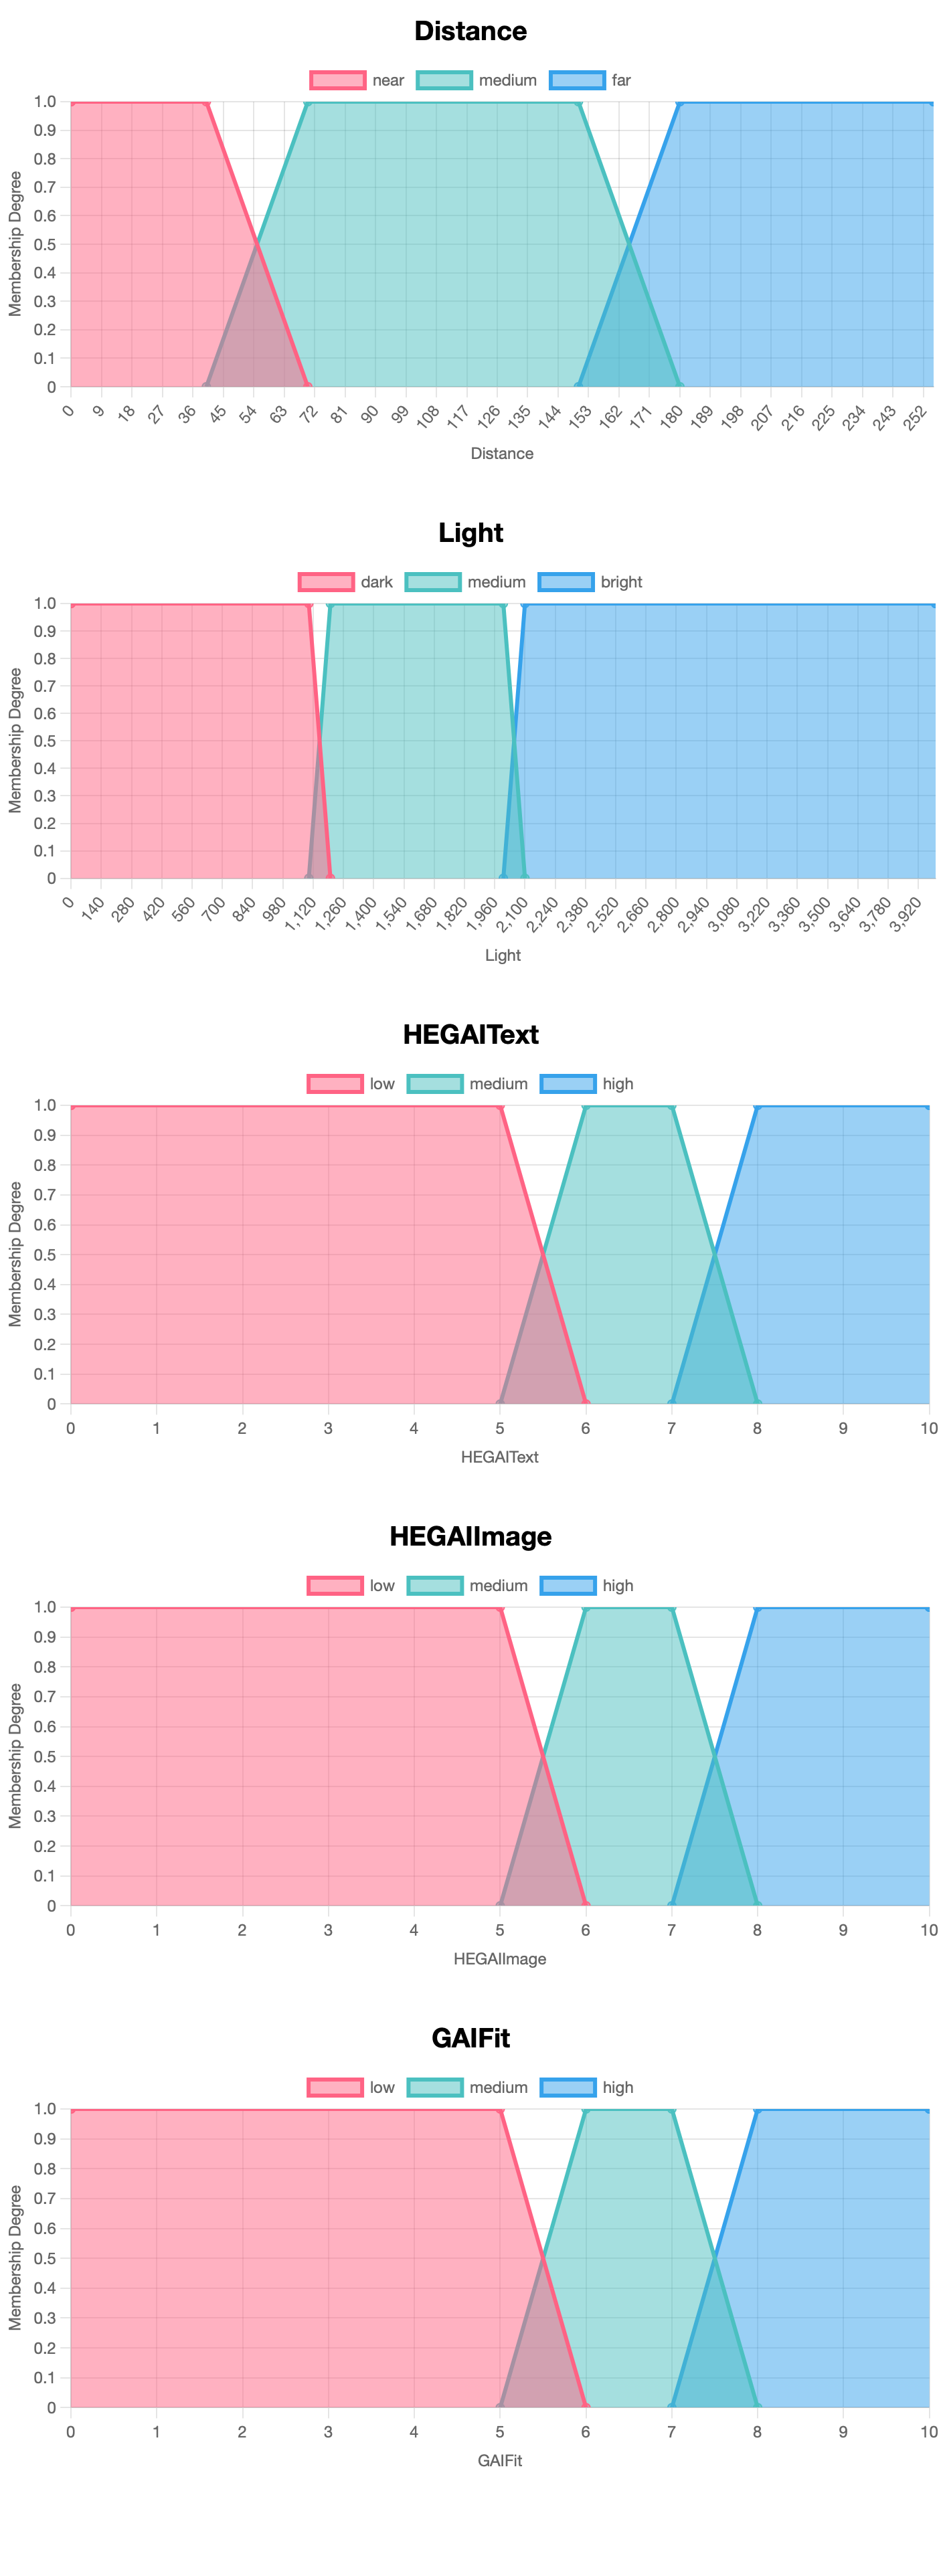
\includegraphics[width=\linewidth]{res/image/all_BT.png}
        \caption{訓練前 T 型圖}
        \label{fig:all_BT}  
    \end{minipage}\hfill % \hfill adds horizontal space between the minipages
    \begin{minipage}[t]{0.48\textwidth}
        \centering
        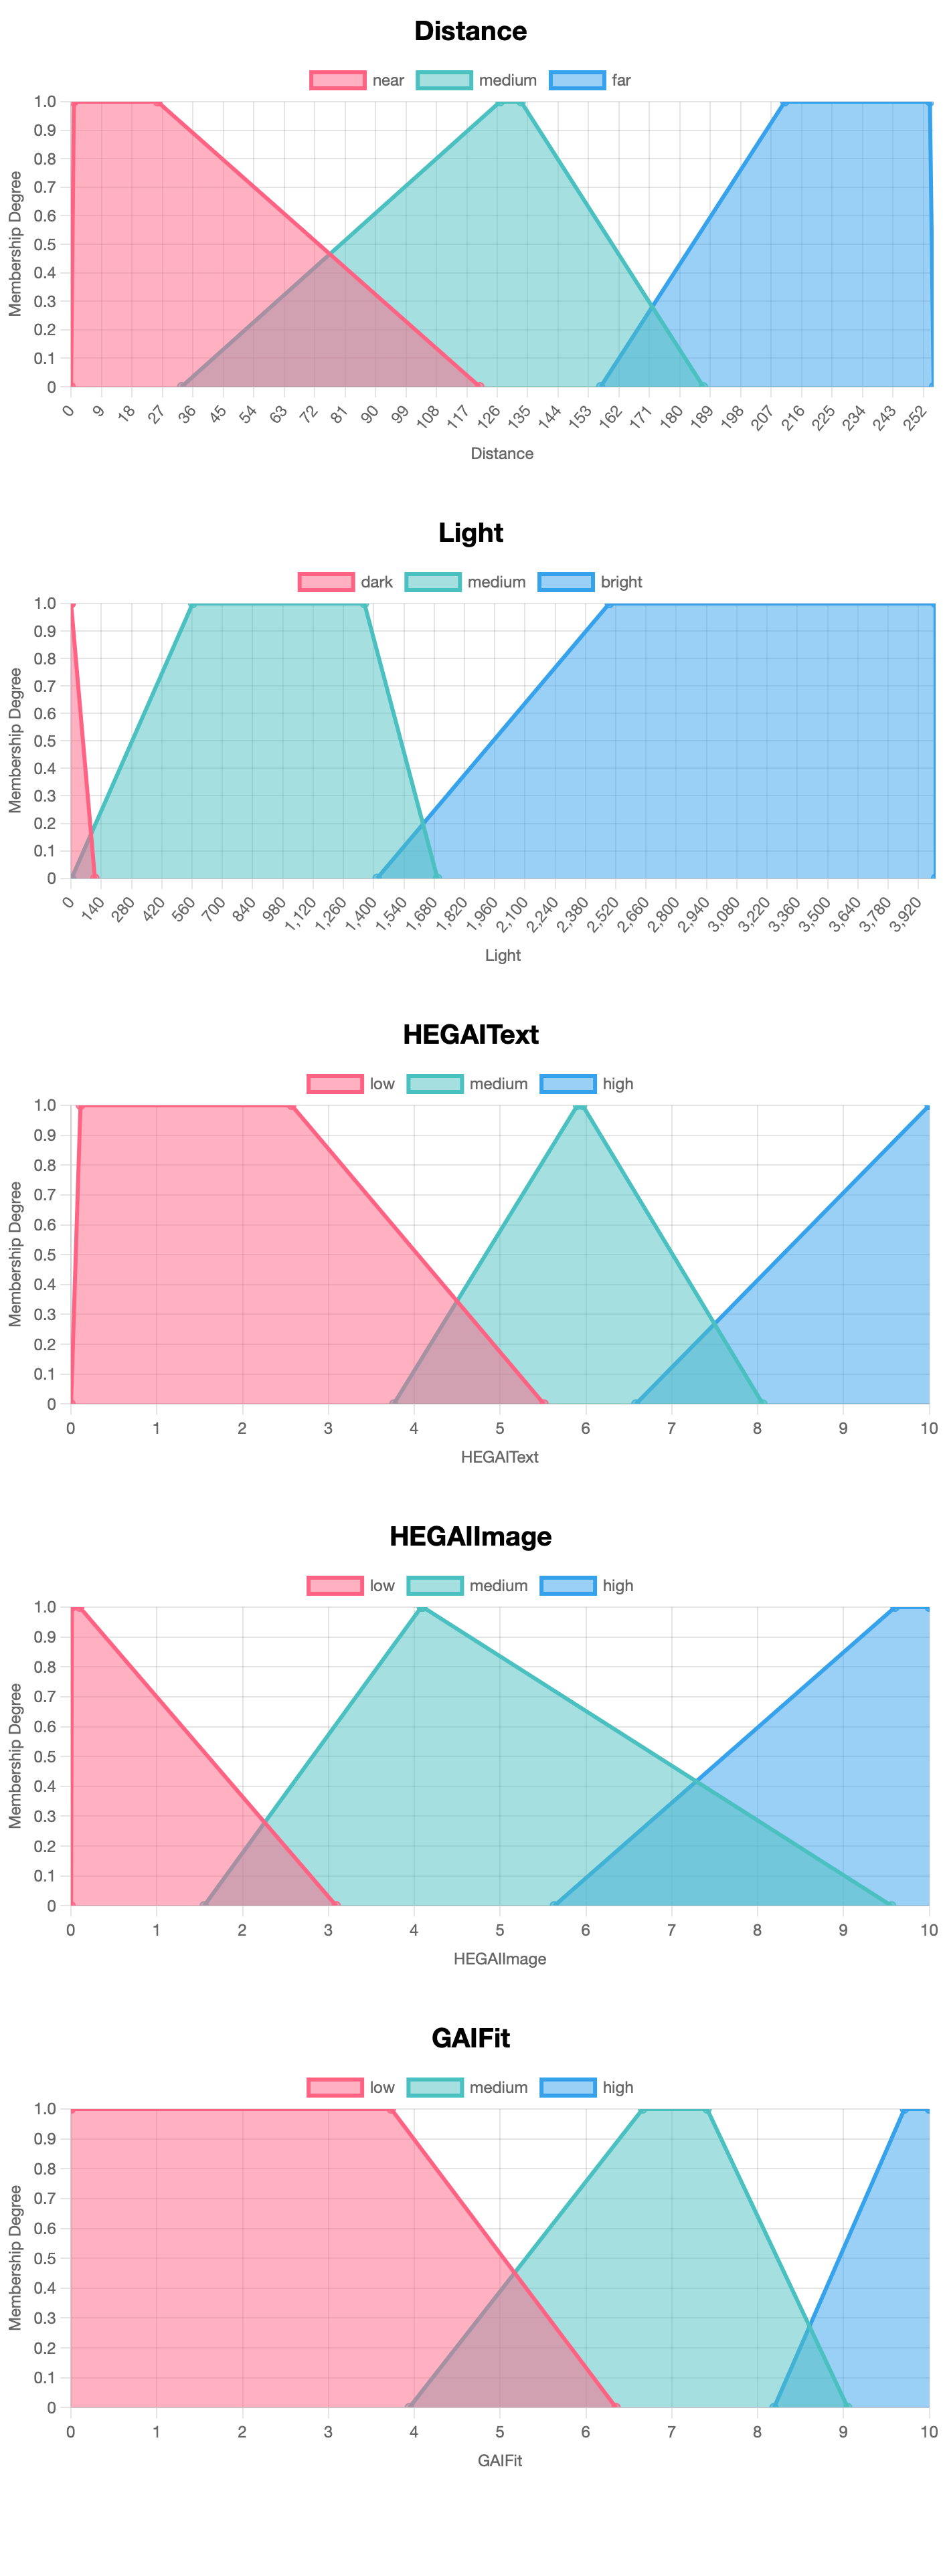
\includegraphics[width=\linewidth]{res/image/all_AL.png}
        \caption{訓練後 T 型圖} % Corrected caption from "訓練會" to "訓練後"
        \label{fig:all_AL}  
    \end{minipage}
\end{figure*}

\begin{figure}[htbp]
    \centering
    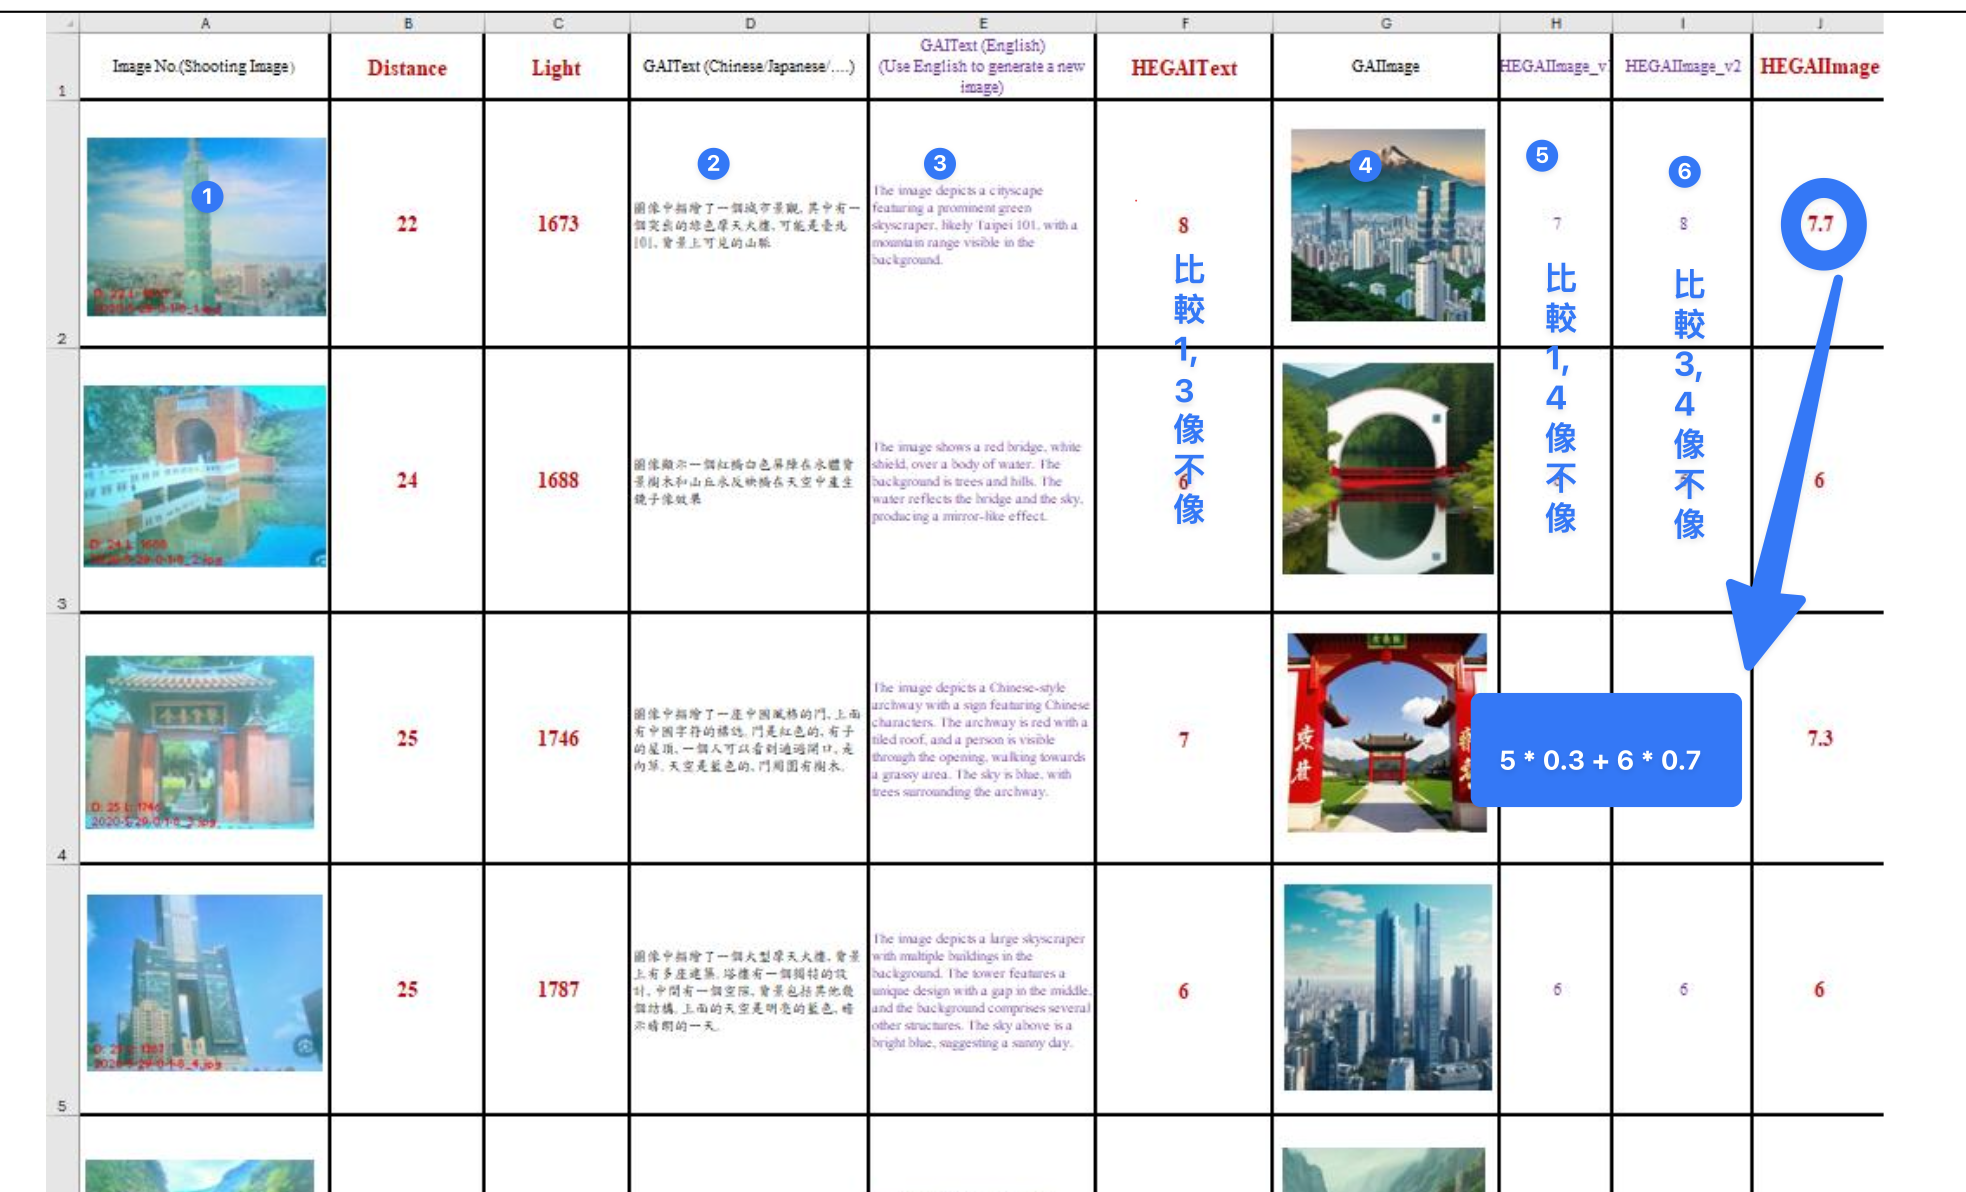
\includegraphics[width=0.45\textwidth]{res/image/labeling_train_data.png}
    \caption{學習資料標記}
    \label{fig:labeling_dataset}
\end{figure}
\begin{figure}[htbp]
    \centering
    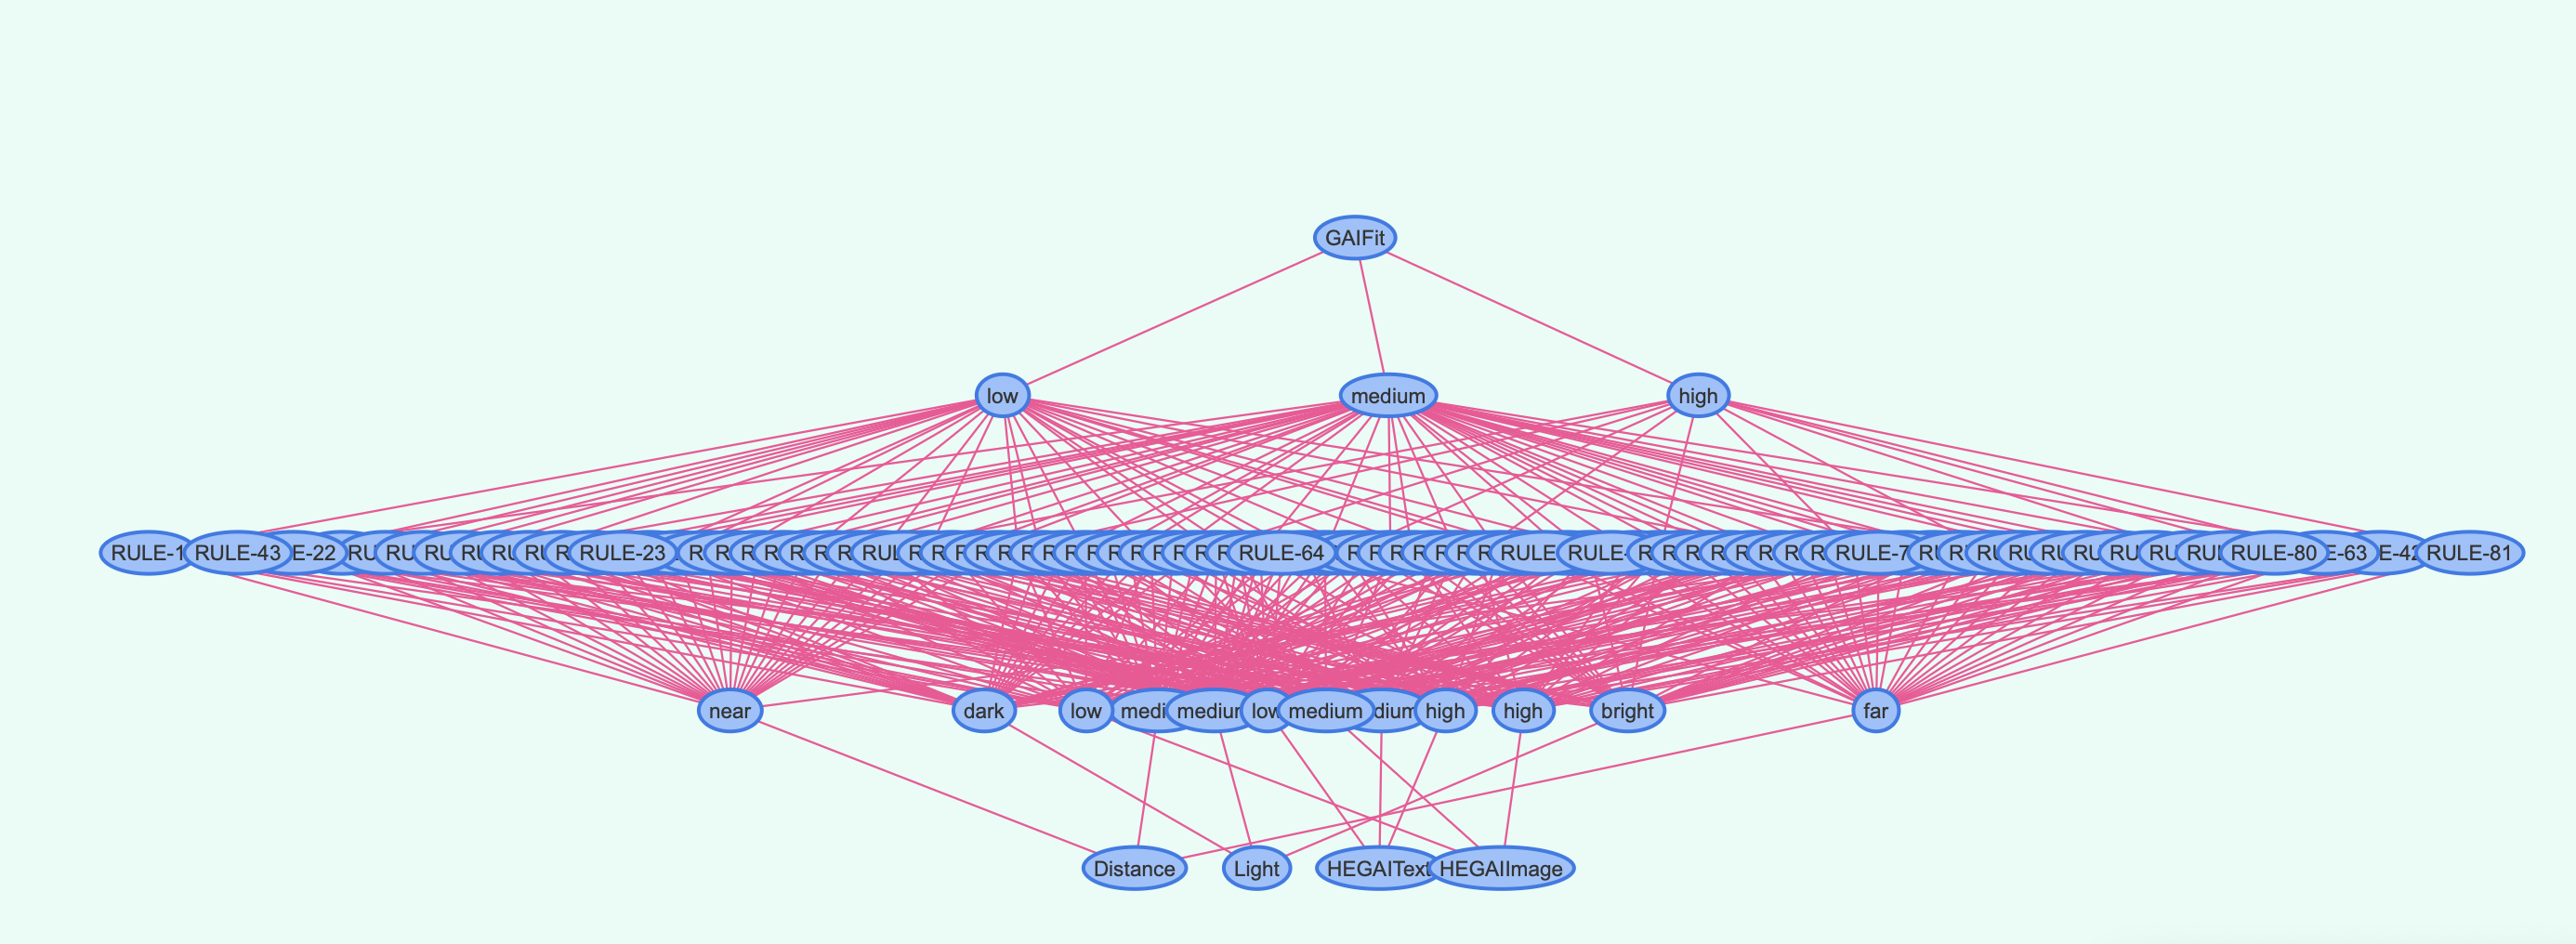
\includegraphics[width=0.45\textwidth]{res/image/model.png}
    \caption{模型}
    \label{fig:model}
\end{figure}

\begin{figure}[htbp]
    \centering
    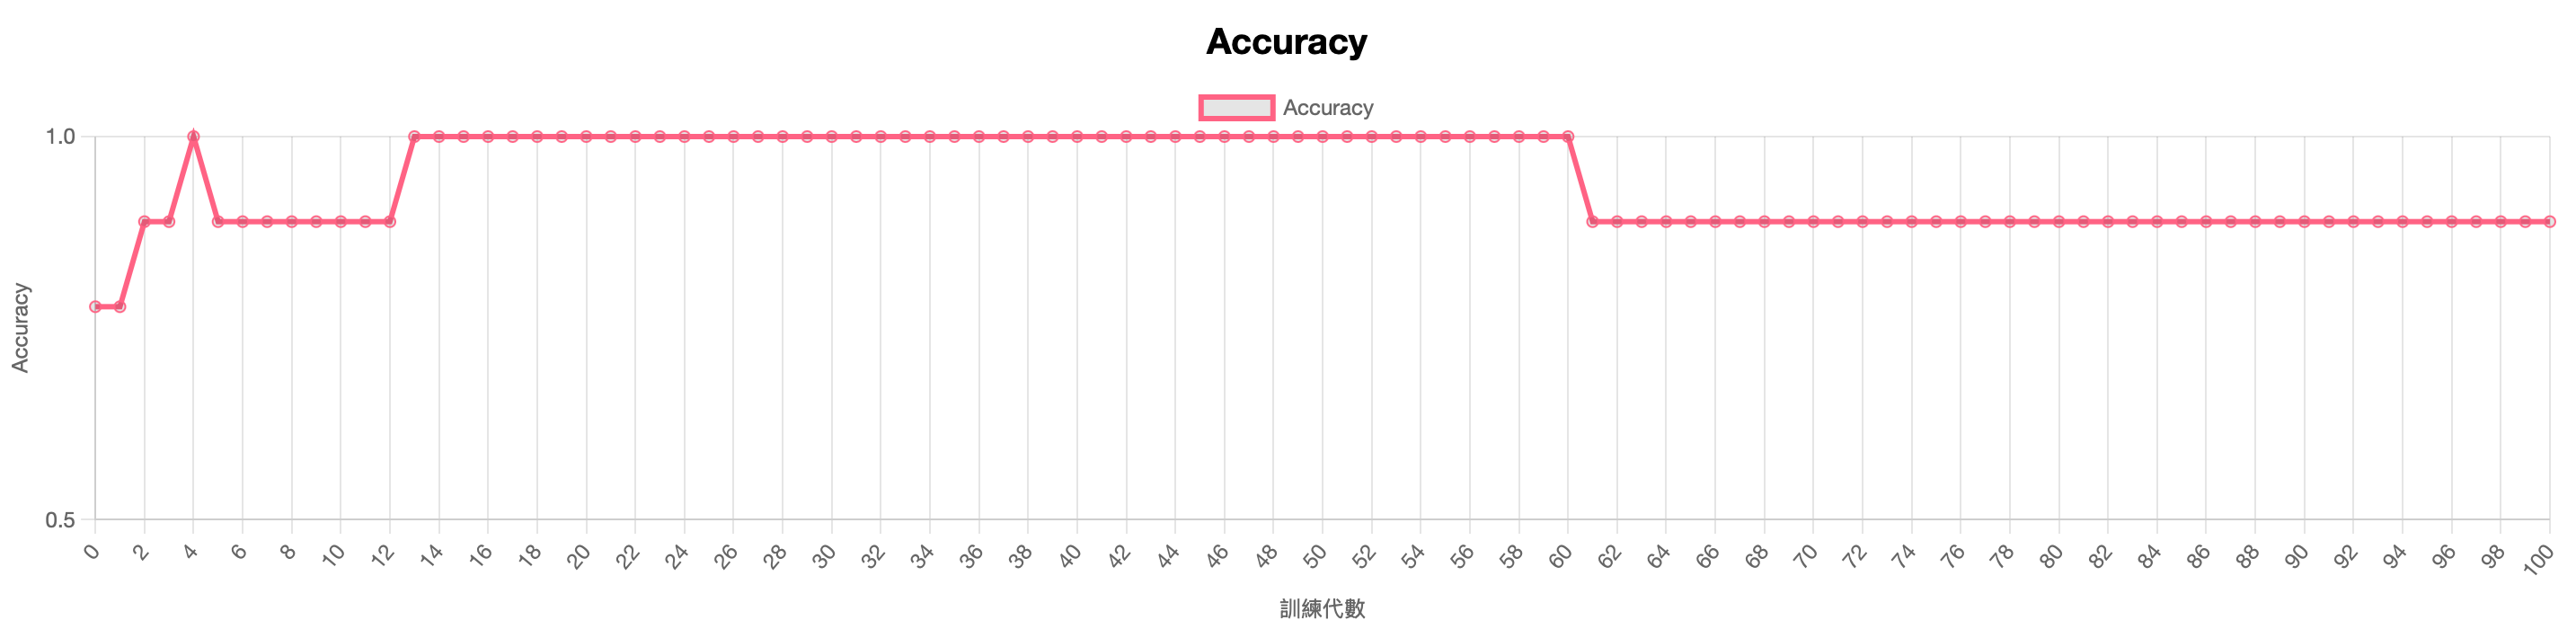
\includegraphics[width=0.45\textwidth]{res/image/accuracy.png}
    \caption{Accuracy Curve}
    \label{fig:accuracy_curve}
\end{figure}
\begin{figure}[htbp]
    \centering
    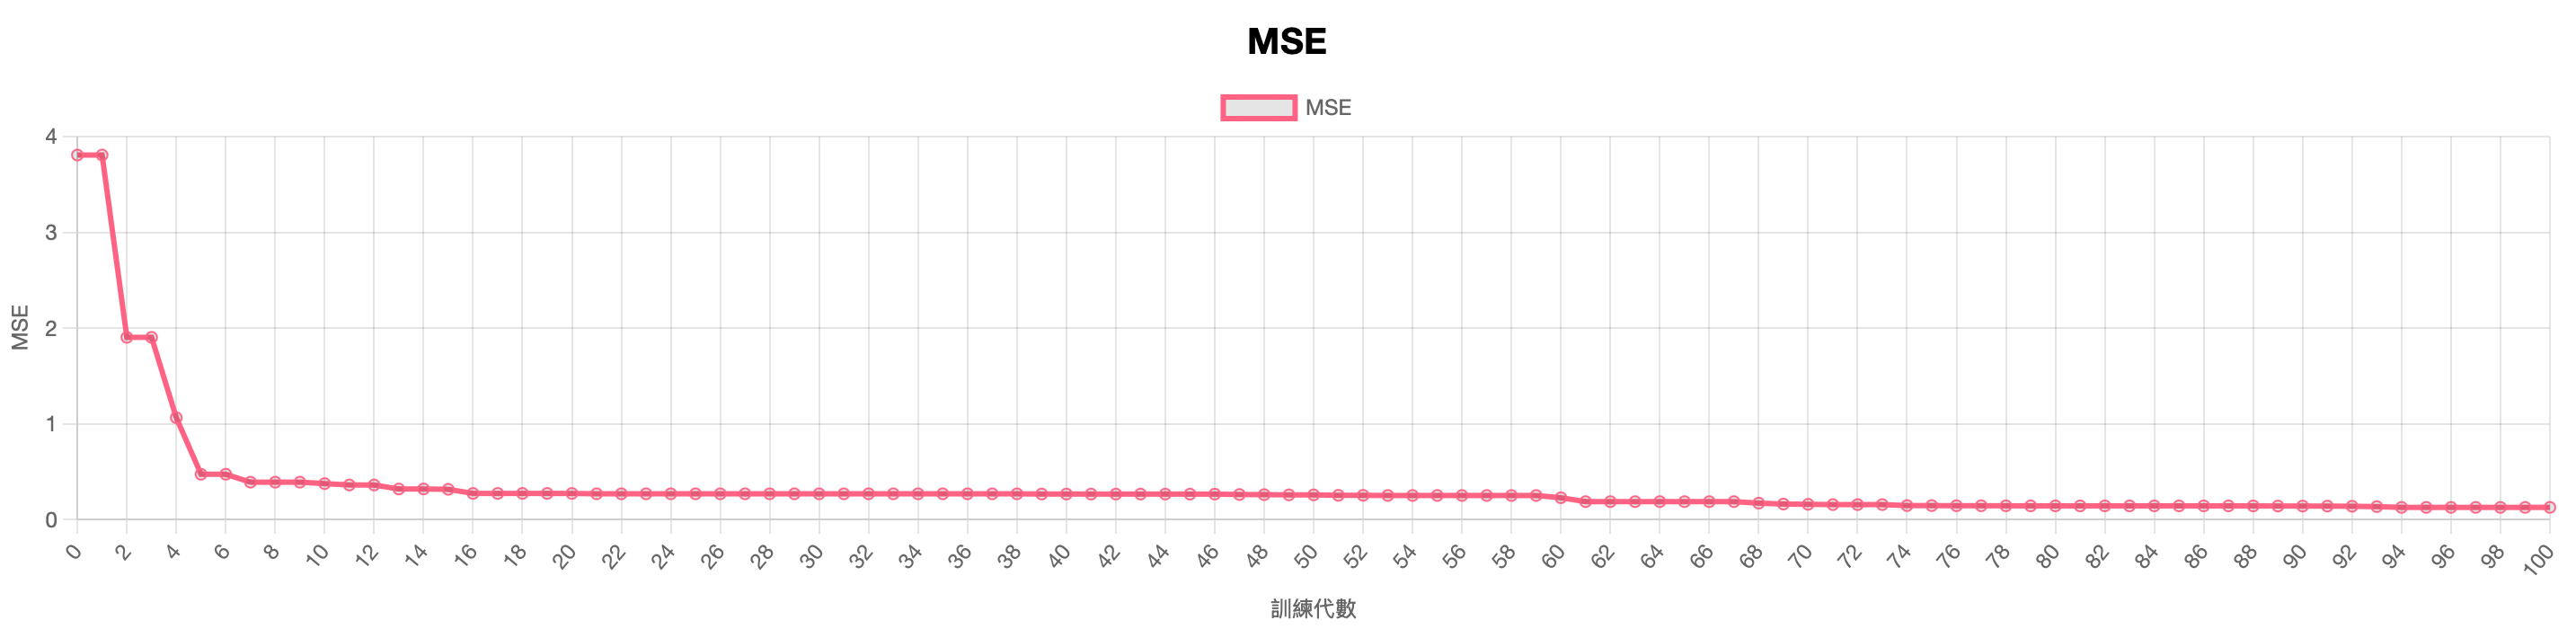
\includegraphics[width=0.45\textwidth]{res/image/mse.png}
    \caption{MSE Curve}
    \label{fig:mse_curve}
\end{figure}
\begin{figure}[htbp]
    \centering
    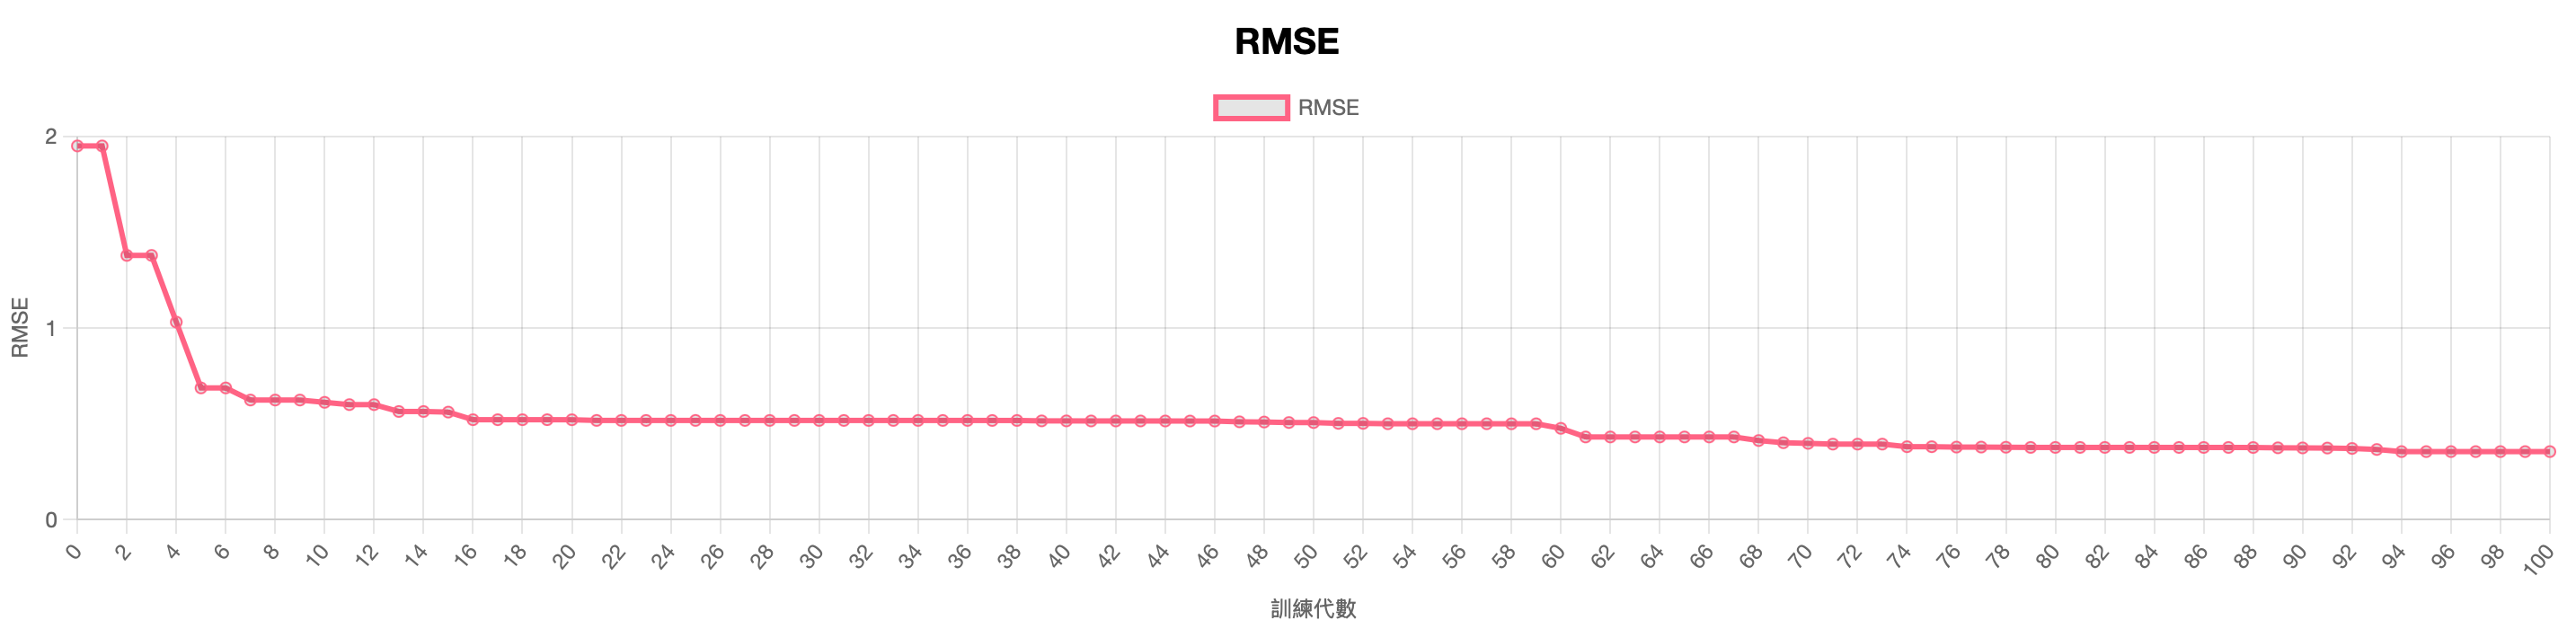
\includegraphics[width=0.45\textwidth]{res/image/rmse.png}
    \caption{RMSE Curve}
    \label{fig:rmse_curve}
\end{figure}
\begin{figure}[htbp]
    \centering
    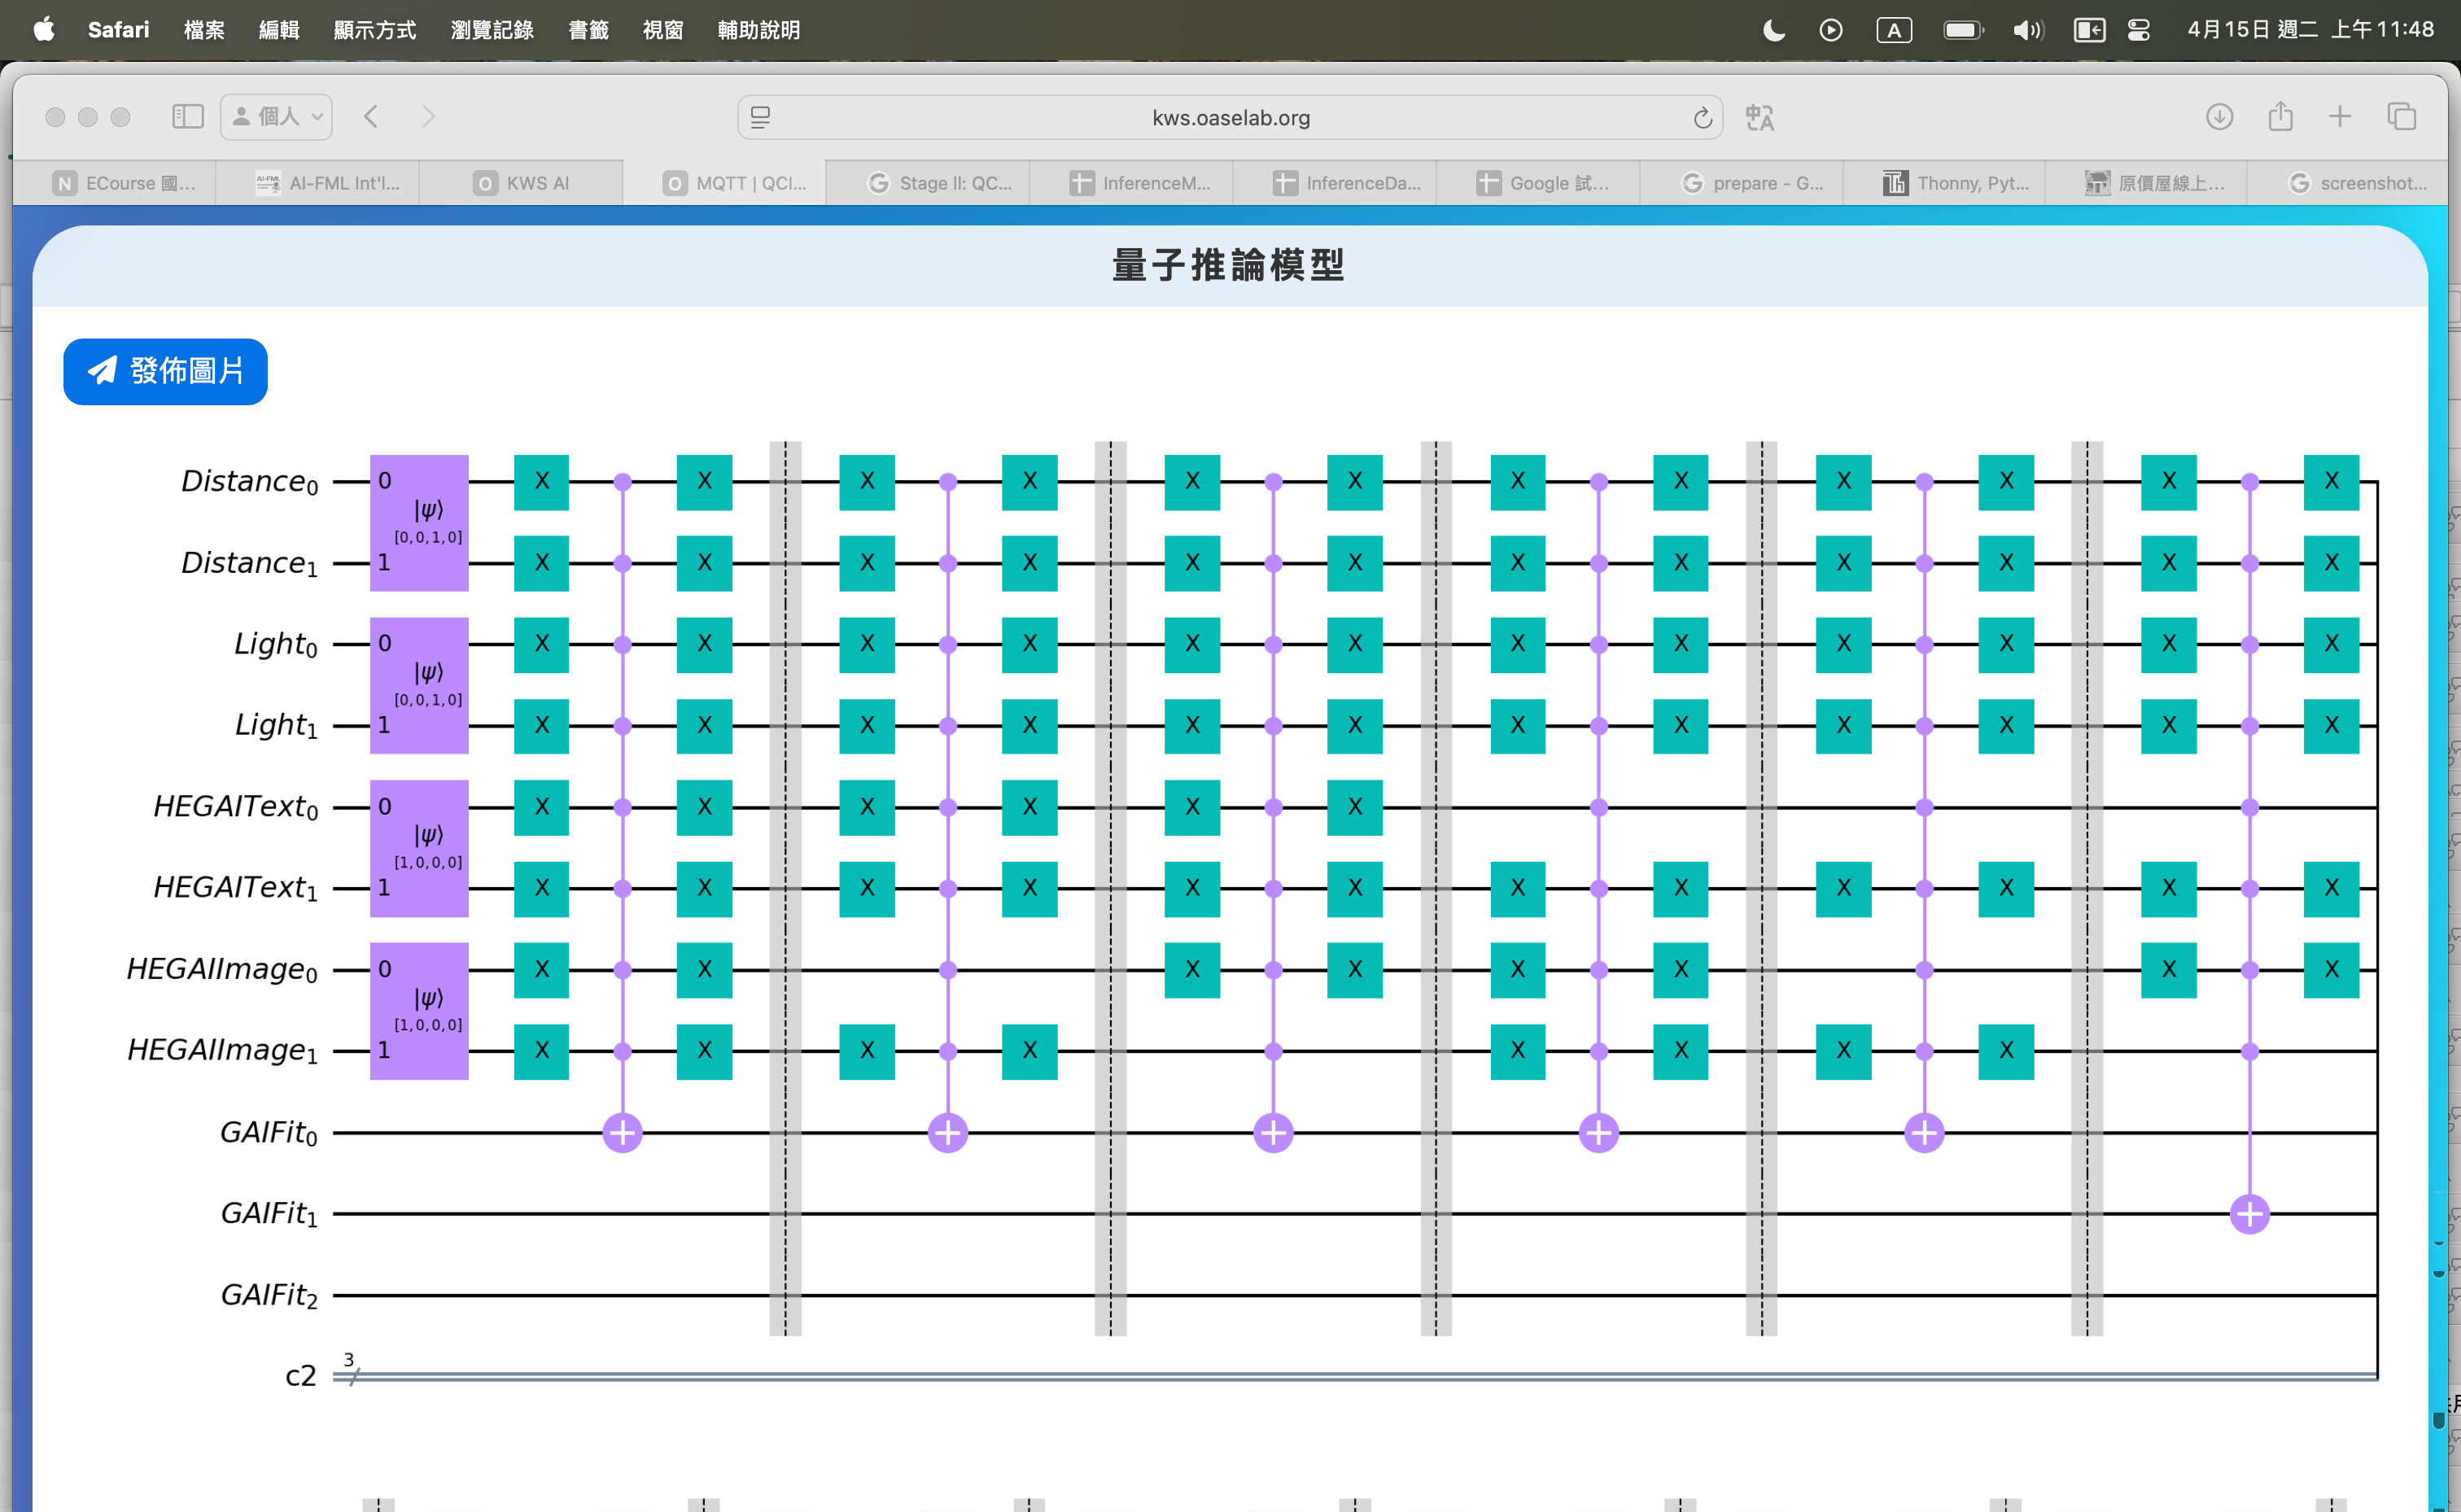
\includegraphics[width=0.45\textwidth]{res/image/quantum.png}
    \caption{量子電路實現}
    \label{fig:quantum_circuit}
\end{figure}


\FloatBarrier

\section{軟體工程LLM軟體應用(Macro/Meso/Micro)}
本節探討 LLM 技術 (以 KUWA+TAIDE+RAG 系統為例) 在 Software Engineering 實踐中不同層次的應用。

\subsection{Macro 層次應用 (策略與規劃)}
在 Macro 層次,LLM 可輔助 Software Project Management 和早期 Requirements Elicitation。例如,利用 LLM 分析市場趨勢、生成初步的專案提案、識別潛在風險,或快速草擬 User Stories。RAG 功能可以整合行業報告或標準文件,為決策提供依據。

\subsection{Meso 層次應用 (設計與開發輔助)}
在 Meso 層次,LLM 可作為開發團隊的助手。例如,輔助 Software Design(生成程式碼框架、API 文件草稿)、協助程式碼撰寫與除錯 (Debugging)、自動生成 Unit Tests,或解釋複雜的既有程式碼。Kuwa 平台的多模型 Room 功能有助於比較不同 LLM 在特定開發任務上的表現。

\subsection{Micro 層次應用 (個人生產力提升)}
在 Micro 層次,個別開發者可利用 LLM 提升個人工作效率。例如,快速查詢技術問題、學習新的程式語言或框架、潤飾技術文檔、生成 commit messages 或輔助撰寫郵件。本地部署的 TAIDE 模型確保了在無網路或處理敏感資訊時的可用性。

\subsection{KUWA+TAIDE+RAG 專案時程圖}
以下為 KUWA+TAIDE+RAG 環境建置與初步應用專案的簡化時程圖佔位符。
% Placeholder for KUWA+TAIDE+RAG schedule figure
\begin{figure}[htbp]
    \centering
    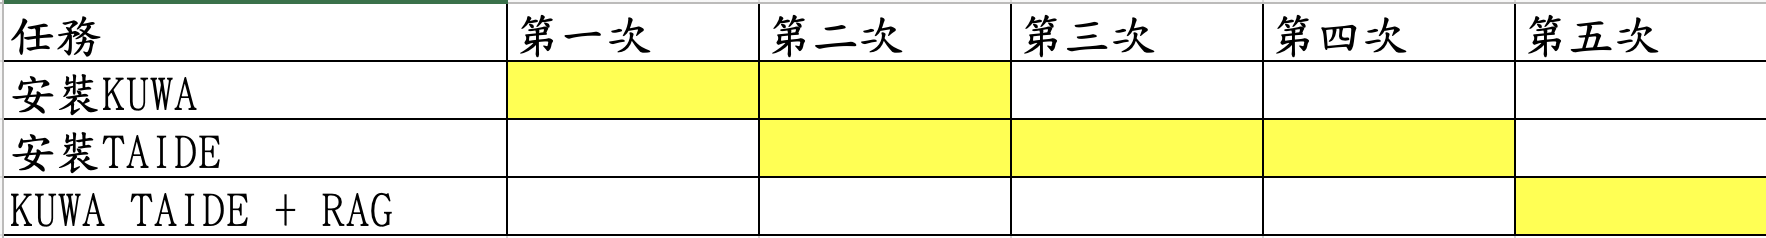
\includegraphics[width=0.45\textwidth]{res/image/kuwa_timeline.png} % Example
    \caption{KUWA+TAIDE+RAG 專案時程圖示例}
    \label{fig:kuwa_schedule}
\end{figure}
\FloatBarrier

\section{軟體工程QCI\&AI軟硬體整合應用(Macro/Meso/Micro)}
本節探討 QCI\&AI 軟硬體整合技術在 Software Engineering 實踐中不同層次的應用。

\subsection{Macro 層次應用 (前瞻性研究與系統架構)}
在 Macro 層次,QCI\&AI 整合應用主要體現在對具有潛在高影響力問題的前瞻性研究,例如優化複雜系統、新材料發現的模擬等,這些可能催生全新的軟體架構 (Software Architecture) 需求。Software Engineering 方法可確保這些探索性專案的系統性與可管理性。

\subsection{Meso 層次應用 (特定演算法與工具開發)}
在 Meso 層次,QCI\&AI 的整合應用促使開發針對特定量子演算法或模糊邏輯系統的軟體工具與函式庫。本報告中描述的 QCI\&AI 學習工具即為一個實例,其開發過程遵循了 Software Development Life Cycle (SDLC) 的諸多階段,從 Data Collection 到模型驗證 (Model Validation) 和硬體互動。

\subsection{Micro 層次應用 (實驗與學習平台)}
在 Micro 層次,QCI\&AI 軟硬體平台為研究人員和學生提供了進行實驗、學習量子概念和 AI 演算法的實踐環境。透過實際操作硬體並觀察結果,可以深化對抽象理論的理解,這對於培養下一代 QCI\&AI 軟體工程師至關重要。

\subsection{QCI\&AI 軟硬體整合專案時程圖}
以下為 QCI\&AI 軟硬體學習工具開發與實驗專案的簡化時程圖佔位符。
% Placeholder for QCI&AI schedule figure
\begin{figure}[htbp]
    \centering
    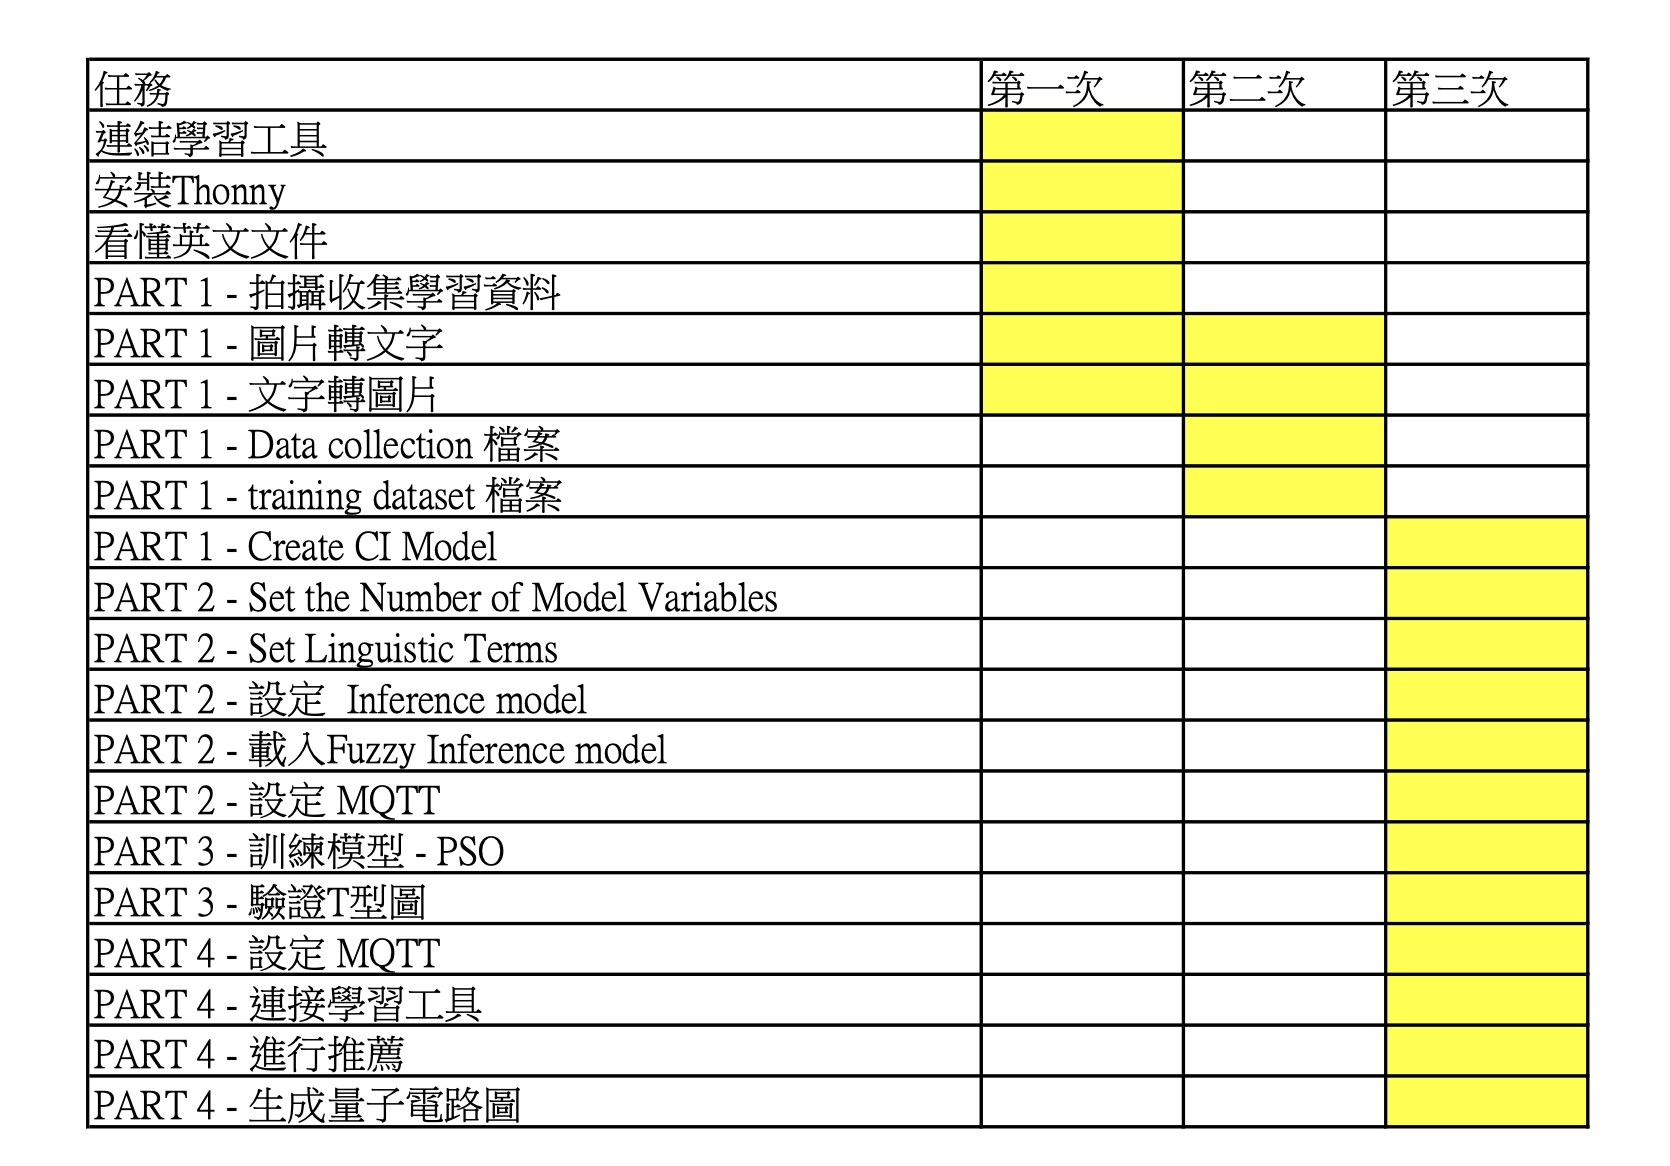
\includegraphics[width=0.45\textwidth]{res/image/QCI_AI_timeline.png} % Example
    % \fbox{\parbox[c][20em][c]{0.45\textwidth}{\centering 預留位置: \\ QCI\&AI 軟硬體整合專案時程圖 (甘特圖) \\ (包含主要階段:硬體設定、資料收集框架開發、模糊邏輯模型實現、演化算法整合、量子推理模塊開發、測試與驗證)}}
    \caption{QCI\&AI 軟硬體整合專案時程圖示例}
    \label{fig:qciai_schedule}
\end{figure}
\FloatBarrier

\section{生成式AI對我學習軟體工程分析}
我覺得在我學習的過程中是正面的,
有時候生成式AI的回答不一定正確,
常常會有幻覺產生的情況,
讓我學會了如何去查證這些資料的正確性,
所以我覺得生成式AI可以幫助我更快的理解軟體工程的概念,
這些工具不僅能加速我的學習過程,還能激發我對於軟體開發的興趣和創造力。

% \textit{本節請您根據個人經驗,詳細闡述生成式 AI (Generative AI) 工具(如本報告中使用的 LLM 及 Kuwa 平台)在您學習 Software Engineering 過程中帶來的正面影響、負面影響以及整體性的評估。例如:}
% \begin{itemize}
%     \item \textit{\textbf{正面影響:} 是否加速了對 Software Engineering 概念的理解?是否有助於程式碼撰寫、除錯或文檔編寫?是否激發了新的學習興趣或專案想法?}
%     \item \textit{\textbf{負面影響:} 是否可能導致過度依賴?是否擔心資訊的準確性?在學習初期使用是否會妨礙基礎能力的培養?}
%     \item \textit{\textbf{整體影響與未來展望:} 總體而言,Generative AI 對您的 Software Engineering 學習之路是助力還是阻力?您認為未來 Software Engineering 教育應如何整合這些 AI 工具?}
% \end{itemize}

\noindent 心得影片: \url{https://youtu.be/spqwshHfivA} \\


\section*{致謝}
本報告的完成,誠摯感謝指導教授李健興博士在
Software Engineering 與 QCI\&AI 領域的專業指導和啟發。
同時,特別感謝國立臺南大學與國立高雄大學以及國家高速網路計算中新提供的學術資源與支持環境。
對於 KuwaAI 團隊提供的 KUWA 及 TAIDE 團隊提供的 LLaMA-TAIDE 3.1 8B 模型 以及好心人提供的 LLaMA-TAIDE 3.1 8B Q4 KM 量化的 模型
使得本報告的實作部分得以順利進行,在此表達由衷謝意。
最後,感謝所有提供建議的同學們以及幫助我的助教們,沒有他們我無法完成這份報告。

% References
\begin{thebibliography}{9}

\bibitem{llama_taide}
{TAIDE Project Team}, ``{TAIDE Llama 3.1 Large Language Model},'' {Taiwan}, {2024} (Year is an estimate, please update). [Online]. Available: \url{https://taide.tw/index}
\bibitem{li2013ch1}
李允中, ``軟體工程:第一章 軟體危機與流程,'' 國立臺灣大學資訊工程學系, 臺北, 2013.

\bibitem{li2013ch2}
李允中, ``軟體工程:第二章 需求工程,'' 國立臺灣大學資訊工程學系, 臺北, 2013.

\bibitem{li2013ch3}
李允中, ``軟體工程:第三章 物件導向軟體開發,'' 國立臺灣大學資訊工程學系, 臺北, 2013.

\bibitem{li2013ch4}
李允中, ``軟體工程:第四章 軟體設計,'' 國立臺灣大學資訊工程學系, 臺北, 2013.

\bibitem{kuwa_github}
KuwaAI, *GenAI OS*. [Online]. Available: \url{https://github.com/kuwaai/genai-os}. Accessed: May 13, 2025.

\end{thebibliography}


\end{document}